\chapter{Аналитический раздел}
\label{cha:analysis}
\section{Постановка задачи}
В соответствии с заданием на выпускную квалификационную работу магистра требуется разработать метод для управления памятью в многопоточных приложениях.
Для решения поставленной задачи необходимо:
\begin{itemize}
	\item проанализировать существующие методы выделения виртуальной памяти приложениям;
	\item проанализировать существующие способы выделения физической памяти приложениям;
	\item разработать метод выделения памяти, сокращающий накладные расходы при выделении памяти;
	\item разработать алгоритм распределения памяти и структуру ПО;
	\item провести исследование разработанного метода.
\end{itemize}

\subsection{Отображение памяти}
Наименьшая единица выделения памяти в современных операционных системах - страница\cite{page}. Ее размер обычно равен 4КБ, но есть, так называемые, большие страницы, размер которых варьируется на каждой архитектуре и для x86 состовляет 2МБ. Этот размер ограничен базовым оборудованием. Это означает, что ОС не может запросить памяти меньше чем размер страницы. Процессор не умеет работать с памятью линейно, для получения физического адреса делается запрос в УУП (англ. MMU)\cite{mmu}  (который   по   сути является кешом TLB)\cite{tlb}, если адрес отсутствует, то выполняется обращение к таблицам: от таблицы страниц к таблице указателей на каталоги страниц, и после получает нужный адрес.\cite{wepskam}

Процесс может запросить память у ОС через 2 системных вызова: \textbf{\textit{mmap}}\cite{mmap} и \textbf{\textit{sbrk}}\cite{sbrk}.

\textbf{\textit{sbrk}} управляет точкой разрыва программы, тоесть функция опеределяет доступную процессу память просто инкрементируя указатель на свободную память в куче\cite{heap} до тех пока, пока не достигнет области отображаемой в процесс памяти.

\textbf{\textit{mmap}} отображает в адресное пространство процесса системные страницы памяти.

Почти все существующие библиотеки отказались от использования \textbf{\textit{sbrk}} в пользу \textbf{\textit{mmap}} по следующим причинам:
\begin{itemize}
	\item у sbrk есть ограничение в виде лимита выделения памяти, данный лимит - это ближайшая к нему отображаемая область памяти;
	\item память выделяется только линейно, нельзя выделить в любом месте кучи как это умеет делать mmap.
\end{itemize}

Вызов \textbf{\textit{mmap}} занимает больше времени, но он более гибок и универсален в использовании. Но одними системными вызовами не получится эффективно управлять оперативной памятью. Каждый системный вызов генерирует прерывание, которое приостанавливает код в пространстве пользователя и перемещается   на исполнение кода в пространстве  ядра, это называется сменой контекста. Смена контекста процесса является тяжелой операцией, которая требует сохранить текущее состояние процесса. Поэтому все библиотеки стараются делать эти вызовы как можно реже и запрашивать у ОС как можно больше памяти за один системный вызов.

Физическая страница памяти идентифицируется по номеру фрейма страницы (PFN)\cite{page-frame}. PFN можно легко вычислить по физическому адресу, разделив его на размер страницы (или сдвинув физический адрес с помощью битов \textit{PAGE\_SHIFT} вправо).

\begin{figure}[!h]
	\begin{center}
		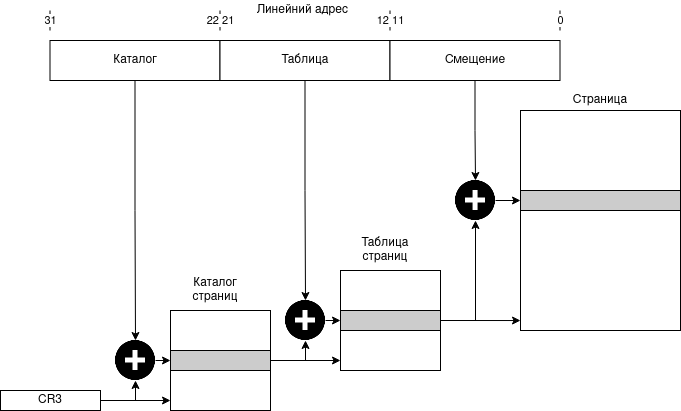
\includegraphics[scale=0.6]{images/memory-mapping.png}
		\caption{Обращение к странице памяти по адресу.}
		\label{memory-mapping}
	\end{center}
\end{figure}

Для повышения эффективности работы с памятью, виртуальное адресное пространство разделено на пространство пользователя и пространство ядра. По той же причине пространство ядра содержит зону отображения памяти, называемую \textbf{низкими адресами} (англ. lowmem), которая последовательно отображается в физической памяти, начиная с наименьшего возможного физического адреса. Виртуальный адрес, по которому отображается \textbf{lowmem}, определяется параметром \textit{PAGE\_OFFSET}. Не вся доступная память может быть отображена в \textbf{lowmem}, и из-за этого в пространстве ядра есть отдельная зона, называемая \textbf{зоной высоких адресов} (англ. highmem), которая может использоваться для произвольного отображения физической памяти. Память, выделенная через \textbf{kmalloc()}, находится в \textbf{lowmem} и физически смежна. Память, выделенная через \textbf{vmalloc()}, не является непрерывной и не находится в lowmem (у нее есть выделенная зона в highmem).\cite{memory-mapping}

\begin{figure}[!h]
	\begin{center}
		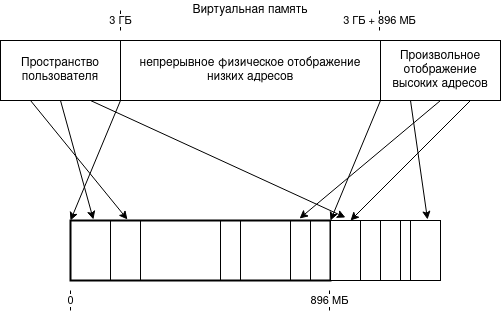
\includegraphics[scale=0.6]{images/virtual-memory.png}
		\caption{Отображение виртуальной памяти в физическую.}
		\label{virtual-memory}
	\end{center}
\end{figure}

\section{Glibc malloc}
Glibc является стандартной библиотекой языка С для систем, построенных на базе ядра Linux. В ней же реализован и стандартный системный аллокатор для програм пользователей, который доступен через интерфейсы malloc/free.

\subsection{Общее описание}
Изначально, в качестве стандартного системного аллокатора, использовалась библиотека dlmalloc, но она не поддерживала работу с потоками, поэтому была заменена на ptmalloc2, которая в дальнейшем стала частью glibc и теперь является стандартным аллокатором памяти. Поддержка работы с потоками помогает повысить производительность аллокатора и, следовательно, производительность приложений. В dlmalloc, когда два потока вызывают malloc одновременно, только один поток может войти в критическую секцию, так как свободный список памяти разделен между всеми потоками. Следовательно, выделение памяти занимает много времени в многопоточных приложениях, что приводит к снижению производительности. В то время как в ptmalloc2, когда два потока вызывают \textbf{\textit{malloc}} одновременно, память выделяется быстрее, так как каждый поток поддерживает отдельный сегмент кучи и для каждой кучи имеется свой список свободной памяти. Процесс поддержания отдельных структур данных кучи и свободного списка для каждого потока называется ареной потока.\cite{glibc-malloc-overview}

\subsection{Арена}
Как уже было сказано, арена это структура данных, которая отвечает за распределение памяти определенному количеству потоков\cite{arena}. Есть два вида арен:
\begin{itemize}
	\item главная арена;
	\item арена под несколько потоков.
\end{itemize}
Главная арена создается основном потоком исполнения и управляет кучей через системный вызов \textbf{\textit{sbrk}}, тогда как потоковая арена запрашивает память у ОС через \textbf{\textit{mmap}}. При этом, если пользователь запросил память размером более чем 128КБ и в текущей куче ее недостаточно для удовлетворения запроса, память выделяется через системный вызов \textbf{\textit{mmap}}, вне зависимости от того в какую арену пришел запрос на выделение. Но выделять отдельную арену под каждый поток может требовать много ресурсов, поэтому они не создаются бесконечно, Поэтому количество активных арен для одного процесса ограничено значениями:
\begin{itemize}
	\item для 32-ух разрядных систем - 2 * количество логических ядер в системе;
	\item для 64-ех разрядных систем - 8 * количество логических ядер в системе.
\end{itemize}
Например, если есть многопоточное приложение (4 потока, основной + 3 пользовательских) запущенное но 32-ух битной системе, на которой есть 1 процессорное ядро. Количество потоков, в данном случае, больше лимита арен, которое доступно процессу на этом ПК (4 > 2 * 1). В таком случае библиотека должна гарантировать разделение арен между несколькими потоками:
\begin{itemize}
	\item основной поток исполнения вызывает \textbf{\textit{malloc}}, используется уже созданная главная арена без каких-либо блокировок;
	\item потоки 1 и 2 вызывают \textbf{\textit{malloc}}, для каждого создается отдельная арена без каких-либо блокировок, на данный момент количество арен равно количеству потоков;
	\item поток 3 вызывает \textbf{\textit{malloc}}, лимит арен на процесс в системе достигнут, поэтому \textbf{\textit{malloc}} попробует переиспользовать уже созданные арены:
	\begin{itemize}[$\star$]
		\item идет линейный проход по всем аренам, в этот момент производится попытка захватить мьютекс для сериализации доступа;
		\item если удалось захватить ресурс, то память возвращается польpователю (к примеру удалось захватить главную арену);
		\item если не удалось, то произойдет попытка захвата следующей арены.
	\end{itemize}
	\item теперь, когда 3-ий поток вызвал \textbf{\textit{malloc}} 2-ой раз, тот попытается переиспользовать арену, которая была испольщована в предыдущий раз (в данном случае это главная арена), еслт она недоступна, поток блокируется до тех пор, пока арена не освободится, получается что главная арена разделена между основном и 3-им потоками.
\end{itemize}

\subsection{Множественные кучи}
В библиотеке есть 3 основных структуры данных:
\begin{itemize}
	\item \textit{heap\_info}, заголовок кучи, одна арена потока может иметь несколько куч, каждая куча имеет свой собственный заголовок, потому что они состоят из разных отображаемых областей, и у каждой такой области будет свой заголовок;
	\item \textit{malloc\_state}, заголовок арены, у одной арены может быть множество куч, но для них всех определен только один заголовок арены;
	\item \textit{malloc\_chunk}, заголовок блока, куча разделена на множество блоков и у каждого есть свой заголовок.
\end{itemize}
У главной арены нет множества куч и поэтому нет и структуры \textit{heap\_info}, когда главная арена заканчивается, то инкреметрируется указатель разрыва программы до тех пор, пока не упрется в область отображаемой памяти. В отличии от потоковой арены, заголовок арены главной арены - это глобальная переменная, которую можно найти в сегменте данных файла libc.so.

\begin{figure}[!h]
	\begin{minipage}{0.5\textwidth}
		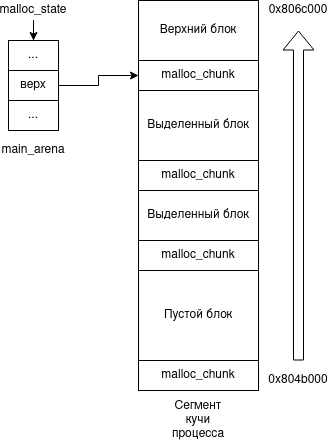
\includegraphics[scale=0.5]{images/glibc-malloc-main-arena.png}
		\caption{Диаграмма главной арены.}
		\label{glibc-malloc-main-arena}
	\end{minipage}
	\begin{minipage}{0.5\textwidth}
		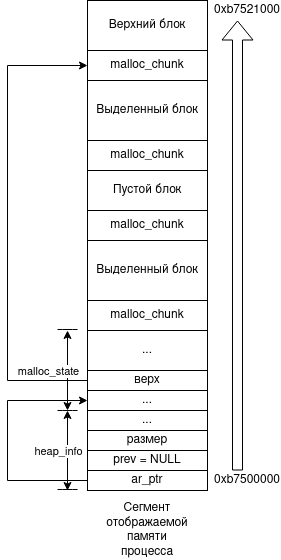
\includegraphics[scale=0.4]{images/glibc-malloc-thread-arena.png}
		\caption{Диаграмма потоковой арены.}
		\label{glibc-malloc-thread-arena}
	\end{minipage}
\end{figure}

\begin{figure}[!h]
	\begin{center}
		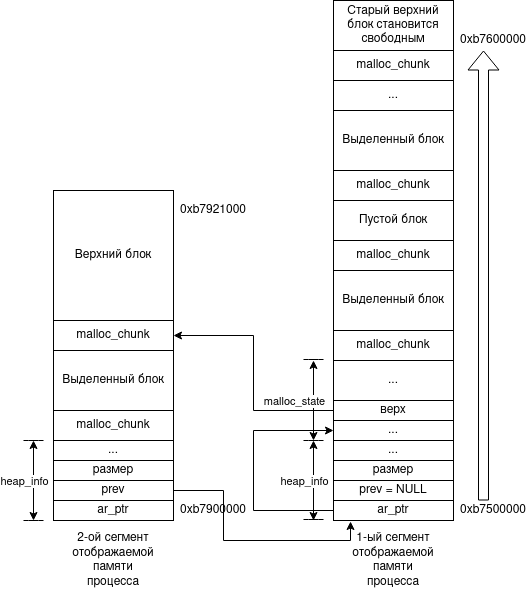
\includegraphics[scale=0.6]{images/glibc-malloc-thread-arena-multi.png}
		\caption{Диаграмма потоковой арены с несколькими кучами.}
		\label{glibc-malloc-thread-arena-multi}
	\end{center}
\end{figure}

\subsection{Блоки}
Есть несколько типов блоков, которые можно найти в сегменте кучи:
\begin{itemize}
	\item выделенный блок;
	\item свободный блок;
	\item верхний блок;
	\item последний блок.
\end{itemize}

\bigbreak
\textbf{\textit{Выделенный блок}}

\textit{\textbf{prev\_size}} - если предыдущий фрагмент свободен, то это поле содержит размер предыдущего фрагмента. В противном случае, если выделен предыдущий фрагмент, это поле содержит пользовательские данные предыдущего фрагмента.

\textit{\textbf{size}} - это поле содержит размер выделенного фрагмента. Последние 3 бита этого поля содержат информацию о флаге.
\begin{itemize}
	\item \textbf{PREV\_INUSE(P)} - этот бит устанавливается при выделении предыдущего блока;
	\item \textbf{IS\_MAPPED(M)} - этот бит выставлен если блок является отображаемым в память процесса через \textbf{\textit{mmap}};
	\item \textbf{NON\_MAIN\_ARENA(N)} - этот бит выставлен когда блок принадлежит потоковой арене.
\end{itemize}
Другие поля \textit{malloc\_chunk} (например, fd, bk) не используются для выделенного фрагмента. Следовательно, вместо этих полей хранятся пользовательские данные. Запрошенный пользователем размер преобразуется в полезный размер (внутренний размер представления), так как требуется некоторое дополнительное пространство для хранения \textit{malloc\_chunk}, а также для целей выравнивания. Преобразование происходит таким образом, что последние 3 бита полезного размера никогда не задаются и, следовательно, используются для хранения информации о флаге.

\bigbreak
\textit{\textbf{Свободный блок}}

\textit{\textbf{prev\_size}} - никакие два свободных блока не могут соседствовать друг с другом, когда оба блока свободны, оин объединяется в один свободный блок большего размера. Следовательно, всегда будет выделен предыдущий фрагмент для этого освобожденного фрагмента, и поэтому \textit{prev\_size} содержит пользовательские данные предыдущего фрагмента.

\textit{\textbf{size}} - это поле содержит размер свободного блока.

\textit{\textbf{fd}} (forward pointer) - указывает на следующий фрагмент в той же ячейке (а не на следующий фрагмент, присутствующий в физической памяти).

\textit{\textbf{bk}} (backward pointer) - указывает на предыдущий фрагмент в той же ячейке (а не на предыдущий фрагмент, присутствующий в физической памяти).

\begin{figure}[!h]
	\begin{minipage}{0.5\textwidth}
		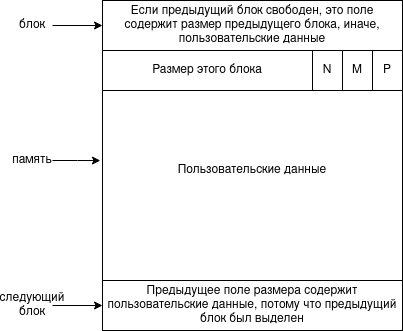
\includegraphics[scale=0.5]{images/glibc-malloc-allocated-chunk.png}
		\caption{Выделенный блок.}
		\label{glibc-malloc-allocated-chunk}
	\end{minipage}
	\begin{minipage}{0.5\textwidth}
		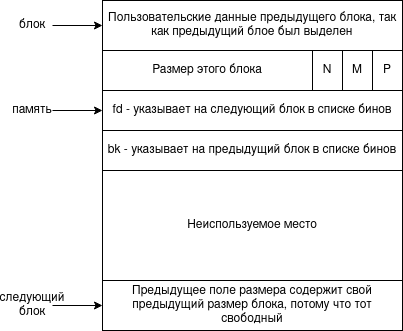
\includegraphics[scale=0.5]{images/glibc-malloc-free-chunk.png}
		\caption{Свободный блок.}
		\label{glibc-malloc-free-chunk}
	\end{minipage}
\end{figure}

\subsection{Бины}
Бины это структуры данных в свободном списке, которые хранят свободные блоки. В зависимости от размеров блоков, есть несколько типов бинов:
\begin{itemize}
	\item быстрые бины;
	\item неотсортированные бины;
	\item малые бины;
	\item большие бины.
\end{itemize}

В библиотеке есть 2 структуры данных, которые хрянят эти бины:
\begin{itemize}
	\item fastbinsY - этот массив содержит быстрые бины;
	\item bins - этот массив содержит неотсортированные, малые и большие бины, всего их 126 и они разделены следующим образом: 1-ый бин - неотсортированный, бины со 2-го по 63-ий - малые, бины с 64-го по 126-ой - большие.
\end{itemize}

\bigbreak
\textit{\textbf{Быстрые бины}}

Блоки размером от 16 до 80 байт называются быстрами. Ячейки, которые содержат такие блоки называются быстрыми бинами. Среди всех видом ячеек, быстре бины быстрее всего выделяют и освобождают память.

\begin{figure}[!h]
	\begin{center}
		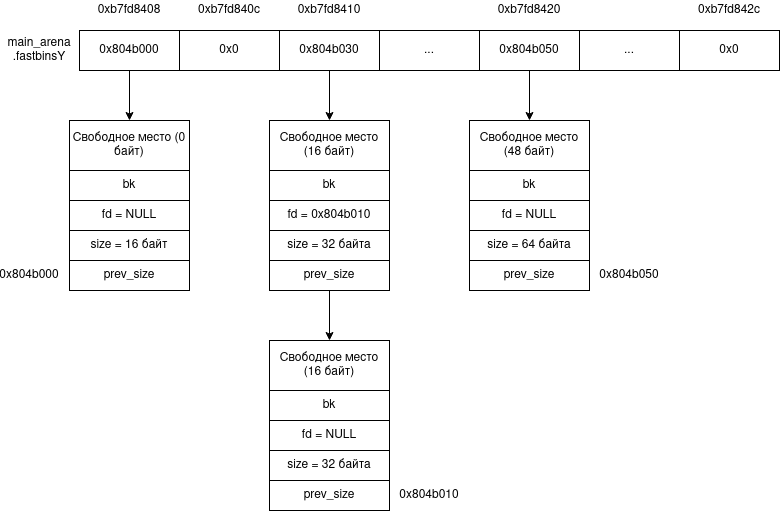
\includegraphics[scale=0.6]{images/glibc-malloc-fast-bin-snap.png}
		\caption{Список быстрых бинов.}
		\label{glibc-malloc-fast-bin-snap}
	\end{center}
\end{figure}

\bigbreak
\textit{\textbf{Неотсортированные бины}}

Когда малый или большой блоки освобождаются, они добавляются в список неотсортированных бинов. Такой подход позволяет библиотеке переиспользовать недавно освобожденные блоки. Поэтому скорость выделения и освобождения памяти немного возрастает, потому что исчезает время на поиск подходящего бина.

\begin{figure}[!h]
	\begin{center}
		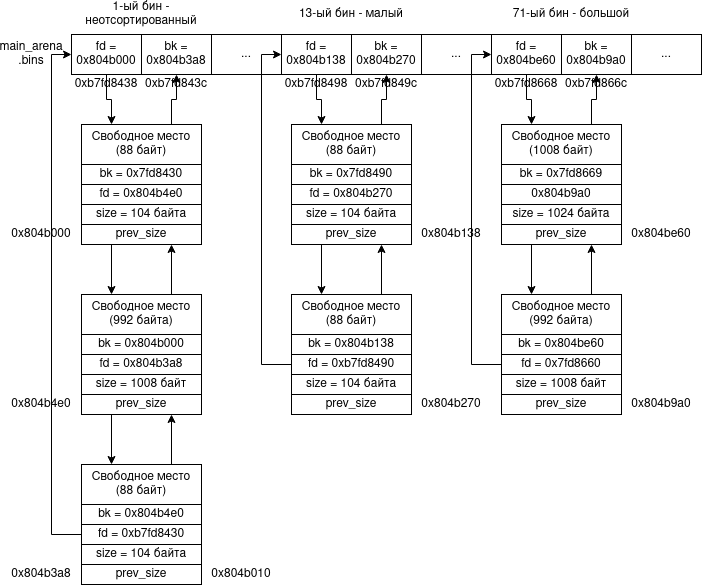
\includegraphics[scale=0.6]{images/glibc-malloc-all-bins.png}
		\caption{Список неотсортированный, мылых и больших бинов.}
		\label{glibc-malloc-all-bins}
	\end{center}
\end{figure}

\bigbreak
\textit{\textbf{Малые бины}}

Блоки размером менее чем 512 байт называются малыми. Бины, содержащие маоые блоки, называются малыми бинами. Малые бины быстрее чем большие, но медленнее чем быстрые в выделении и освобождении памяти.

\textit{\textbf{Большие бины}}

Блоки размером более чем 512 байт называются большими. Бины, которые соджержат большие блоки, называются большими бинами. Эти бины выделяют память медленнее всего.

\textit{\textbf{Верхний блок}}
	
Блок, находящийся на верхней границе арены, называется верхним блоком. Он не принадлежит ни одному бину и используется для обработки запроса пользователя когда нет свободных блоков ни в одном из бинов. Если размер верхнего блока больше чем запрашиваемый пользователем, он делится на 2 блока:
\begin{itemize}
	\item пользовательский блок нужного размера;
	\item оставшаяся часть блока.
\end{itemize}
Оставшийся блок становится новым верхним блоком, если его размер менее чем запрашиваемый польщователем, память увеличивается через вызов \textit{\textbf{sbrk}} (главная арена) или \textit{\textbf{mmap}} (потоковая арена).

\textit{\textbf{Последний оставшийся блок}}

Это оставшийся блок после последнего разделения. Он позволяет улучшить локальность ссылки, тоесть последовательные запросы на выделение памяти могут оказаться выделенными рядом. Последним оставшимся блоком называется тот, который, в случае когда пользовательский запрос не может быть выполнен с использованием неотсортированного или малого бинов, тогда список больших бинов сканируется для того, чтобы найти следующий по величине не пустой бин. Когда такой блок найден, он разбивается на 2, польщовательский блок возвращается польщователю, а остаток помешается в список неотсортированных бинов и становится последним оставшемся блоком. Теперь, когда польщователб будет последовательно запрашивать малые блоки и последний оставшейся блок является единственным блоков в списке неотсортированных бинов, он разбивается на 2 блока, один вернется пользователю, другой станет новым оставшимся блоком и помещается в список неотсортированных бинов. Поэтому последовательные аллокации оказываются рядом друг с другом.

\section{TCMalloc}
TCMalloc\cite{tcmalloc-design-doc} это аллокатор памяти, разработанный компанией Google и являющийся заменой стандартному системному аллокатору, он имеет следующие характеристики:
\begin{itemize}
	\item Быстрое выделение и освобождение памяти для большинста объектов. Обекты кэшируются в зависимости от режима, либо кэш в каждом потоке, либо кэш на логический процессор. Большинство аллокаций не требуют синхронизации доступа к ресурсам, благодаря этому конкуренция за выделение памяти сводится к минимуму и обеспечивает хорошее масштабирование для многопоточных приложений.
	\item Гибкое использование памяти, освобожденная память может быть переиспользована для объектов различных размеров или возвращена системе.
	\item Низкие накладные расходы на память под каждый объект за счет выделения ``страниц'' объектов одинакового размера. Это позволяет хранить небольшие объекты в памяти эффективно и помогает избежать излишней фрагментации памяти.
	\item Низкая стоимость сэмлирования, которое позволяет получить детальное представление об использовании памяти приложением.
\end{itemize}

\subsection{Общее описание}
\begin{figure}[!h]
	\begin{center}
		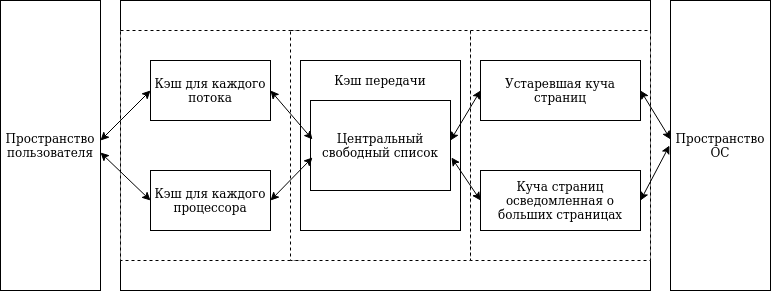
\includegraphics[scale=0.6]{images/tcmalloc-overview.png}
		\caption{Внутренняя структура TCMalloc.}
		\label{tcmalloc-overview}
	\end{center}
\end{figure}

Библиотеку TCMalloc можно разбить на 3 основных компонента. Фронт-энд (англ. front-end), миддл-энд (англ. middle-end) и бэк-энд (англ. back-end):
\begin{itemize}
	\item Фронт-энд является кэшом, который предоставляет быстрое выделение и освобождение памяти приложению.
	\item Миддл-энд отвечает за наполнение фронт-энд кэшей.
	\item Бэк-энд управляет памятью, которая выделяется приложению самой ОС.
\end{itemize}

Фронт-энд может использоваться как в режиме кэш на каждый поток, так и в режиме кэш на каждый логический процессор. Бэк-энд может поддерживать работу с кучей, которая осведомлена о больших страницах.

\subsection{TCMalloc фронт-энд}
Фронт-энд обрабатывает запрос на выделение памяти определенного размера. У него имеется кэш памяти, который может использоваться для выделения или хранения свободной памяти. Этот кэш доступен только одному потоку одновременно, поэтому никаких блокировок не требуется и большинство выделений и освобождений памяти выполняются быстро.

Фронт-энд удовлетворит любой запрос, если у него есть закэшированная память соответствующего размера. Если кэш для этого конкретного размера пуст, будет сделан запрос на пополнение кэша в миддл-энд, который включает в себя центральный список свободной памяти и кэш передачи.

Если миддл-энд исчерпан или запрошенный размер больше максимального размера, который кэшируется фронт-эндом, запрос будет переадресован бек-энду, чтобы либо удовлетворить большое выделение памяти, либо пополнить кэш в миддл-энде. Бэк-энд также называется кучей страниц (англ. pageheap).

На данный момент существует 2 реализации фронт-энда:
\begin{itemize}
	\item Первоначально он поддерживал кэширование объектов по каждому потоку (отсюда и название англ. Thread Caching Malloc). Однако это могло приводить к появлению больних областей памяти, которые масштабировались с увеличением количества потоков. Современные приложения могут иметь большое количество потоков, что приводит либо к большим объемам памяти для каждого потока, либо к тому, что многие потоки имеют крошечные локальные кэши.
	\item Совсем недавно TCMalloc начал поддерживать режим кэширования под каждый логический процессор. В этом режиме каждый процессор в системе имеет свой собственный кэш, из которого выделяется память. Примечание: На x86 логический процессор эквивалентен гиперпотоку.
\end{itemize}

Различия между режимами работы кешей по потокам и процессорам полностью ограничиваются реализациями malloc/new и free/delete.

\textit{\textbf{Выделение памяти под большие и малые объекты}}

Размер на выделение памяти под малые объекты сопоставляется c одним из 60-80 распределяемых размерных классов. Например, выделение 12 байт будет округлено до 16-ти байтового класса размера. Размерные классы предназначены для минимизации объема памяти, который тратится впустую при округлении до следующего по величине размерного класса.

При компиляции с  \_\_STD CPP\_DEFAULT\_NEW\_ALIGNMENT\_\_ <= 8 используется набор размеров, выровненных по 8-ми байтам. Это меньшее выравнивание сводит к минимуму потери памяти для многих распространенных размеров распределения (24, 40 и т.д.), которые в противном случае округляются до кратного 16-ти байтам. Во многих компиляторах это поведение контролируется флагом \textbf{\textit{-fnew-alignment=...}}. Когда \_\_STD CPP\_DEFAULT\_NEW\_ALIGNMENT\_\_ не указан (или больше 8 байт), использются стандартные 16-ти байтовые выравнивания для \textit{\textbf{::operator new}}. Однако при выделении менее 16-ти байт может быть возвращен объект с меньшим выравниванием, так как ни один объект с большим требованием выравнивания не может быть выделен в пространстве.

Когда запрашивается объект заданного размера, запрос сопоставляется с определенным размерным классом с помощью функции \textit{\textbf{SizeMap::GetSizeClass()}}, и возвращаемая память принадлежит этому классу. Это означает, что возвращаемая память по крайней мере так же велика, как и запрошенный размер. Выделения памяти из размерных классов обрабатываются фронт-эндом.

Объекты размером больше предела, определенного максимальным размером (\textbf{kMaxSize}), выделяются непосредственно из бэк-энда. Как таковые они не кэшируются ни фронт ни миддл эндами. Запросы на выделение больших размеров объектов округляются до размера страницы TCMalloc.

\bigbreak
\textit{\textbf{Освобождение памяти}}

Когда объект освобождается, компилятор предоставляет размер объекта, если он известен во время компиляции. Если размер не известен, он будет найден на карте страницы. Если объект мал, он будет помещен обратно в кэш фронт-энда. Если объект больше \textbf{\textit{kMaxSize}}, он возвращается непосредственно в кучу страниц.

\bigbreak
\textit{\textbf{Режим кэша под каждый процессор}}

В этом режиме выделяется один большой блок памяти. На следующей диаграмме показано как этот блок памяти разделен между процессорами и как каждый процессор использует часть блока для хранения метаданных, а также указателей на доступные объекты.

\begin{figure}[!h]
	\begin{center}
		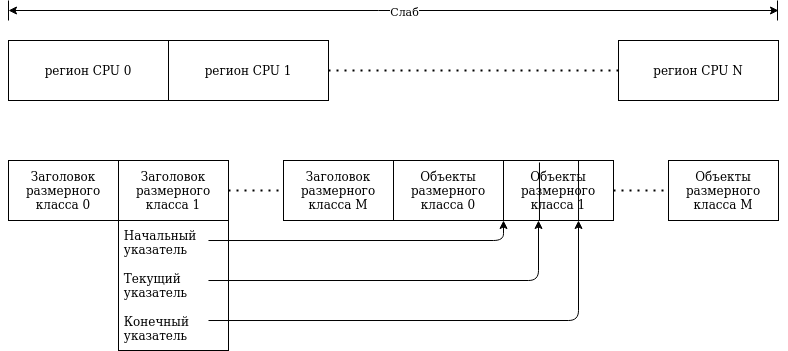
\includegraphics[scale=0.6]{images/tcmalloc-per-cpu.png}
		\caption{Диграмма блока памяти при работе кэша в режиме под каждый процессор.}
		\label{tcmalloc-per-cpu}
	\end{center}
\end{figure}

Каждому логическому процессору назначается секция этой памяти для хранения метаданных и указателей на доступные объекты определенных размерных классов. Метаданные содержат один блок заголовок на каждый размерный класс. Заголовок содержит указатель на начало массива указателей на объекты размерных классов, а также указатель на текущую, динамическую, максимальную емкости и текущую позицию в этом сегменте массива. Статическая максимальная емкость каждого массива указателей для каждого размерного класса определяется во время запуска разницей между началом массива для этого класса и началом массива для следующего класса.

Во время выполнения максимальное количество элементов определенного размерного класса, которое может храниться в блоке для каждого процессора, будет варьироваться, но оно никогда не может превышать статически определенную максимальную емкость, назначенную при запуске.

Когда запрашивается объект определенного размерного класса, он удаляется из этого массива, а когда объект освобождается, он добавляется в массив. Если массив исчерпан, он снова заполняется запросом на выделение памяти в миддл-энд. Если массив переполняется, партия объектов удаляется из него и возвращается в миддл-энд.

Объем памяти, который может быть закэширован, ограничен для каждого процессора параметром \textbf{\textit{MallocExtension::SetMaxPerCpuCacheSize}}. Это означает, что общий объем кэшиуемой памяти зависит от количества активных кэшей под процессоры. Следовательно, машины с более высоким количеством процессоров могут кэшировать больше памяти.

Чтобы избежать удержания памяти на процессорах, где приложение больше не работает, вызывается функция \textbf{\textit{MallocExtension::ReleaseCpuMemory}}, которая освобождает объекты, хранящиеся в кэшах указанного процессора.

Внутри ЦП распределение памяти управляется по всем размерным классам таким образом, чтобы максимальный объем кэшируемой памяти оставался ниже предельно возможного. Тут стоит обратить внимание что он управляет максимальной суммой, которая может быть закэширована, а не суммой, которая в данный момент кэшируется. В среднем, фактически кэшируемая сумма должна составлять примерно половину лимита.

Максимальная емкость увеличивается в тот момент, когда в размерном классе заканчиваются объекты, а также при извлечении большого количества объектов рассматривается возможность увеличения емкости размерного класса. Емкость размерного класса может быть увеличена до тех пор, пока общая память (для всех размерных классов), которую может содержать кэш, не достигнет предела для каждого процессора или пока емкость этого размерного класса не достигнет жестко заданного предела размера для этого размерного класса. Если класс не достиг жестко заданного предела, то для увеличения емкости он может взять емкость из другого размерного класса на том же процессоре.

\bigbreak
\textit{\textbf{Перезапускаемые последовательности и кэш под каждый процессор}}

Для правильной работы, режим кэш под каждый процессор опирается на перезапускаемые последовательности (man rseq(2))\cite{rseq}. Перезапускаемая последовательность - это просто блок инструкций (на языке ассемблера), во многом похожий на типичную функцию. Ограничение перезапускаемых последовательностей состоит в том, что они не могут записывать частичное состояние в память, конечная инструкция должна быть единственной записью обновленного состояния. Идея перезапускаемых последовательностей заключается в том, что если поток удаляется из процессора (например, переключается контекст) во время выполнения перезапускаемой последовательности, то она будет перезапущена сначала. Следовательно, последовательность либо завершится сразу, либо будет многократно перезапущена, пока не завершится без прерываний. Это достигается без использования каких-либо блокирующих или атомарных инструкций, что позволяет избежать конкуренций за ресурсы в самой последовательности.

Практический смысл этого для TCMalloc заключается в том, что код может использовать перезапускаемую последовательность, такую как \textbf{\textit{TcmallocSlab\_Push}}, для извлечения или возврата элемента в массив для каждого процессора без необходимости блокировки. Перезапускаемая последовательность гарантирует, что либо массив обновляется без прерывания потока, либо последовательность перезапускается, если поток был прерван (например, переключателем контекста, который позволяет другому потоку работать на этом процессоре).

\bigbreak
\textit{\textbf{Устаревший режим кэша под каждый поток}}
	
В режиме кэша под каждый поток TCMalloc назначает каждому потоку локальный кэш. Небольшие выделения удовлетворяются из этого локального кэша. Объекты могут перемещаться между миддл-эндом в кэш для потока и из него по мере необходимости.

Потоковый кэш содержит один односвязный список свободных объектов на каждый размерный класс (так что если существует N размерных классов, то будет N соответствующих связных списков), как показано на следующей диаграмме.

\begin{figure}[!h]
	\begin{center}
		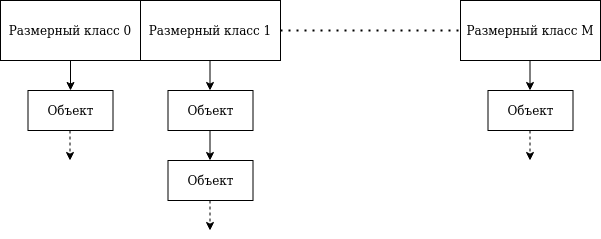
\includegraphics[scale=0.6]{images/tcmalloc-per-thread.png}
		\caption{Диграмма списка свободных объектов при работе кэша в режиме под каждый поток.}
		\label{tcmalloc-per-thread}
	\end{center}
\end{figure}

При выделении объект удаляется из соответствующего размерного класса кэшей для каждого потока. При освобождении объект добавляется к соответствующему списку размерного класса. Переполнение и опустошение обрабатываются путем запроса памяти у миддл-энда или возвращением туда избыточной памяти.

Максимальная емкость кэша для каждого потока устанавливается параметром \textbf{\textit{MallocExtension::SetMaxTotalThreadCacheBytes}}. Однако общий размер может превысить этот предел, так как каждый кэш для каждого потока имеет минимальный размер \textbf{\textit{KMinThreadCacheSize}}, который обычно составляет 512 КБ. В том случае, если поток хочет увеличить емкость своего кэша, ему необходимо уменьшить емкость кэша у других потоков.

По завершению работы потока, вся доступная ему память переходит в миддл-энд в кэш передачи.

\subsection{TCMalloc миддл-энд}
Миддл-энд отвечает за предоставление памяти фронт-энду и возврат памяти в бэк-энд. Он состоит из кэша передачи и центрального свободного списка. Хотя их часто называют сингулярными, существует один кэш передачи и один центральный свободный список на каждый размерный класс. Каждый из этих кэшей защищен мьютексом, поэтому доступ к ним требует затрат на сериализацию.

\bigbreak
\textit{\textbf{Кэш передачи}}

Когда фронт-энд запрашивает или возвращает память, он обращается к кэшу передачи. В нем содержится массив указателей на свободную память, и перемещение объектов в этот массив или извлечение объектов из этого массива по запросу фронт-энда происходят быстро.

Кэш передачи получил свое название из ситуаций, когда один поток выделяет память, освобожденную другим потоком. Он позволяет памяти быстро перемещаться между двумя различными потоками. Если кэш передачи не может удовлетворить запрос памяти или имеет недостаточно места для хранения возвращенных объектов, будет совершено обращение к центральному свободному списку.

\bigbreak
\textit{\textbf{Центральный свободный список}}

Центральный свободный список управляет памятью в спанах (англ. span), спан или диапазон - это набор из одной или нескольких страниц памяти TCMalloc. Запрос на один или несколько объектов удовлетворяется центральным свободным списком путем извлечения объектов из спанов до тех пор, пока запрос не будет удовлетворен. Если в диапазоне недостаточно доступных объектов, то из бэк-энда запрашиваются дополнительные спаны.

Когда объекты возвращаются в центральный свободный список, каждый объект сопоставляется с областью, к которой он принадлежит (с помощью карты страниц), а затем освобождается в эту область. Если все объекты, находящиеся в определенном диапазоне, возвращаются в него, то весь спан возвращается бэк-энду.

\bigbreak
\textit{\textbf{Карты страниц и спаны}}

Куча, управляемая TCMalloc, делится на страницы определенного размера во время компиляции. Область смежных страниц представлена объектом спан. Он может использоваться для управления большим объектом, который был передан приложению, или областью страниц, которые были разделены на последовательность небольших объектов. Если спан управляет малыми объектами, то размерный класс объектов записывается в него.

Карта страниц используется для поиска диапазона, к которому принадлежит объект, или для определения размерного класса для данного объекта. TCMalloc использует 2-ух уровневое или 3-ех уровневое компактное префиксное дерево (англ. radix tree) для отображения всех возможных ячеек памяти на спаны.

На следующей диаграмме показано, как 2-ух уровневая карта страниц используется для отображения адресов объектов на спаны, управляющие системными страницами, в которых находятся объекты. На диаграмме диапазон A занимает две страницы, а диапазон Б 3 страницы.

\begin{figure}[!h]
	\begin{center}
		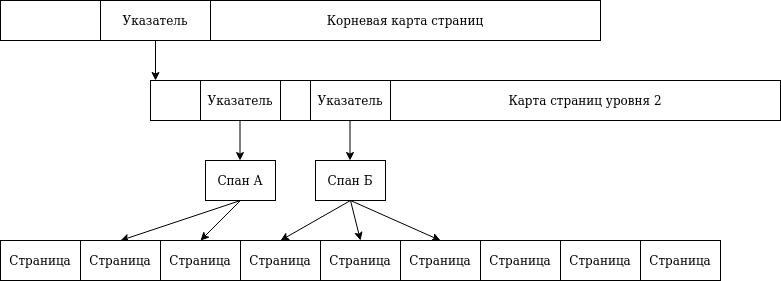
\includegraphics[scale=0.6]{images/tcmalloc-pagemap-and-spans.png}
		\caption{Карта страниц сопоставляет объекты со спанами.}
		\label{tcmalloc-pagemap-and-spans}
	\end{center}
\end{figure}

Спаны используются в миддл-энде для определения места размещения возвращаемых объектов, и в бэк-энде для управления обработкой интервалов страниц.

\bigbreak
\textit{\textbf{Хранение малых объектов в спанах}}
	
Спан содержит указатели на адреса страниц, которыми он управляет. Для небольших объектов эти страницы разделены не более чем на $2^{16}$ объектов. Это значение выбрано таким образом, чтобы в пределах диапазона можно было ссылаться на объекты по двухбайтовому индексу. Это означает, развернутый связный список может быть использован для хранения объектов. Например, если есть 8-ми байтовые объекты, то можно хранить индексы трех готовых к использованию объектов и использовать четвертый слот для хранения индекса следующего объекта в цепочке. Эта структура данных уменьшает пропуски кэша по сравнению с полносвязным списком. Другое преимущество использования двухбайтовых индексов заключается в том, что можно использовать резервную емкость в самом спане для кэширования четырех объектов.

Когда нет доступных объектов определенного размерного класса, необходимо извлечь новый спан из кучи страниц и заполнить его.

\bigbreak
\textit{\textbf{Размеры страниц в TCMalloc}}

TCMalloc можно собрать с различными размерами страниц. Тут стоит отметить что они не соответствуют размерам страниц, которое используются в буффере ассоциативной трансляции (англ. TLB) базового оборудования. Эти размеры страниц в настоящее время составляют 4КБ, 8КБ, 32КБ и 256КБ.

Страница TCMalloc либо содержит несколько объектов определенного размера, либо используется как часть группы для хранения объекта размером больше одной страницы. Если вся страница становится свободной, она будет возвращена бек-энду в кучу страниц и позже может быть перепрофилирована для хранения объектов другого размера (или возвращена в ОС).

Небольшие страницы лучше справляются с требованиями приложения к памяти с меньшими накладными расходами. Например, наполовину использованная страница размером в 4КБ будет иметь 2КБ в остатке по сравнению с 32-ух килобайтной страницей, которая будет иметь 16КБ. Маленькие страницы также с большей вероятностью станут свободными. Например, страница в 4КБ может содержать восемь объектов по 512 байт по сравнению с 64-мя объектами на странице размером в 32КБ; и вероятность того, что 32 объекта будут свободны одновременно, намного меньше, чем вероятность того, что восемь станут свободными.

Большие страницы приводят к уменьшению потребности в извлечении и возврате памяти из бэк-энда. Одна страница размером 32КБ может содержать в восемь раз больше объектов, чем страница размером 4КБ, и это может привести к тому, что затраты на управление большими страницами будут меньше. Кроме того, требуется меньше больших страниц для отображения всего виртуального адресного пространства. TCMalloc имеет карту страниц, которая отображает виртуальный адрес на структуры, управляющие объектами в этом диапазоне адресов. Большие страницы означают, что карта страниц нуждается в меньшем количестве записей и, следовательно, она сама меньше.

Исходя из этого, для приложений с небольшими выделениями памяти или чувствительных к размеру областей памяти, имеет смысл использовать меньшие размеры страниц TCMalloc. Приложения с большим объемом памяти, скорее всего, выиграют от увеличения размеров страниц TCMalloc.

\subsection{TCMalloc бэк-энд }
У бэк-энда в TCMalloc есть 3 задачи:
\begin{itemize}
	\item Управление большими диапазонами неиспользуемой памяти.
	\item Извлечение памяти из операционной системы, когда нет подходящего размера памяти, доступной для выполнения запроса на выделение.
	\item Возврат ненужной памяти обратно в ОС.
\end{itemize}

Существует 2 реализации бэк-энда в TCMalloc:
\begin{itemize}
	\item Устаревшая куча страниц, которая управляет памятью в блоках размером со страницу TCMalloc.
	\item Куча страниц, которой известно о больших страницах, она управляет памятью блоками размером с большую страницу (в данном случае речь идет о размере страницы самого базового оборудования). Управление памятью большими страницами позволяет аллокатору повысить производительность приложения за счет уменьшения пропусков в буффере ассоциативной трансляции.
\end{itemize}

\bigbreak
\textit{\textbf{Устаревшая куча страниц}}

Устаревшая куча страниц - это массив свободных списков для определенных длин смежных страниц доступной памяти. Для всех индексов меньше 256-ти, список по индексу состоит из диапазонов, размер которых равен индексу умноженному на размер страницы TCMalloc. 256-я запись - это список диапазонов, длина которых >= 256 страниц:

\begin{figure}[!h]
	\begin{center}
		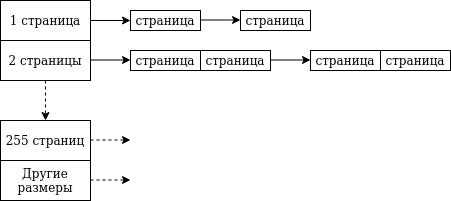
\includegraphics[scale=0.6]{images/tcmalloc-legacy-pageheap.png}
		\caption{Диаграмма устаревшей кучи страниц.}
		\label{tcmalloc-legacy-pageheap}
	\end{center}
\end{figure}

Выделение памяти для N страниц удовлетворяется путем поиска в N-м свободном списке. Если этот свободный список пуст, идет обращение в следующий свободный список и так далее. Если найти нужный диапазон памяти не удается, то память запрашивается у ОС через системный вызов \textbf{\textit{mmap}}.

Если выделение для N страниц удовлетворяется диапазоном страниц длиной большей N, то оставшаяся часть диапазона повторно вставляется обратно в соответствующий свободный список в куче страниц. Когда диапазон страниц возвращается в кучу, соседние страницы проверяются, чтобы определить, образуют ли они теперь непрерывную область, если это так, то страницы объединяются и помещаются в соответствующий свободный список.

\bigbreak
\textit{\textbf{Аллокатор осведомленный о больших страницах}}

Главная цель такого аллокатора - держать память в блоках состоящих из больших системных страниц. На архитектуре x86 размер такой страницы равен 2МБ. Для этого в бэк-энде есть 3 разных кэша:
\begin{itemize}
	\item Кэш наполнителя, содержит большие страницы, из которых была выделена некоторая память. Он имеет сходство с устаревшей кучей страниц в том смысле, что содержит связные списки памяти определенного количества страниц TCMalloc. Запросы на выделение ресурсов размером менее чем больщая страница (как правило) возвращаются из кэша наполнителя. Если кэш наполнителя не имеет достаточного количества доступной памяти, он запросит дополнительные большие страницы.
	\item Кэш регионов, который обрабатывает выделения размером более чем размер большой страницы. Данный кэш позволяет выделениям памяти распределяться между несколькими большими страницами и упаковывать несколько таких выделений в непрерывную область. Это особенно полезно для выделений, которые немного превышают размер огромной страницы (например, 2,1МБ).
	\item Кэш больших страниц обрабатывает выделения памяти размером, по крайней мере, с большую страницу. Существует перекрытие в использовании с кэшом регионов, но кэш регионов включается только тогда, когда точно определено (во время выполнения) что выделение памяти выиграет от этого.
\end{itemize}

\subsection{Рекомендации к использованию}
TCMalloc зарезервирует некоторую память для метаданных при запуске. Количество метаданных будет расти по мере роста кучи. В частности, карта страниц будет расти вместе с диапазоном виртуальных адресов, используемым TCMalloc, а спаны будут расти по мере роста числа активных страниц памяти. В режиме кэшей под каждый логический процессор TCMalloc резервирует блок памяти на процессор (обычно 256КБ), что в системах с большим количеством логических процессоров может привести к многомегабайтным областям в памяти.

Стоит отметить, что TCMalloc запрашивает память у ОС большими порциями (обычно 1ГБ). Адресное пространство зарезервировано, но не резервирует физическую память до тех пор, пока оно не будет использовано. Благодаря такому подходу, виртуальная память приложения (VSS) может быть существенно больше чем резидентная память (RSS). Побочным эффектом этого является то, что попытка ограничить использование памяти приложения путем ограничения VSS, потерпит неудачу задолго до того, как приложение использует столько физической памяти.

Библиотека TCMalloc не создана для того, чтобы использовать ее в уже работающем двоичный файле (например, используя JNI в Java-программах). Двоичный файл выделит некоторые объекты с помощью системного \textbf{malloc} и может попытаться передать их TCMalloc для освобождения. TCMalloc не сможет обрабатывать такие объекты.

\section{Jemalloc}
Проект jemalloc начинался как алокатор памяти для среды выполнения языка программирования, которую Джейсон Эванс разрабатывал в 2005 году, но изменения в дизайне языка сделали его излишним. В то время FreeBSD нуждалась в SMP-масштабируемом аллокаторе, поэтому он интегрировал jemalloc в libc FreeBSD, а затем сделал большое количество улучшений в масштабируемости и поведений фрагментации памяти.

В конце 2007 года проект Mozilla усердно работал над улучшением использования памяти Firefox для версии 3.0, и jemalloc был использован для решения проблем фрагментации Firefox на платформах Microsoft Windows. Многие общие улучшения jemalloc были результатом усилий, связанных с Firefox.

Начиная с 2009 года Джейсон Эванс адаптировал jemalloc для работы с экстремальными нагрузками, в которых обычно работают серверы Facebook, и добавил множество функций, поддерживающих разработку и мониторинг. Facebook использует jemalloc во многих компонентах, которые являются неотъемлемой частью обслуживания его веб-сайта, и по состоянию на 2017 год небольшая команда Facebook ведет постоянную разработку и техническое обслуживание.

Jemalloc - это универсальная реализация вызова \textit{\textbf{malloc}}, которая подчеркивает предотвращение фрагментации и масштабируемую поддержку параллелизма. Библиотека предназначен для использования в качестве системного аллокатора памяти во FreeBSD, но может быть иниегрирована практически в любую среду исполнения. Jemalloc предоставляет множество функций самоанализа, управления памятью и настройки, выходящих за рамки стандартных функций аллокаторов. В качестве крайнего примера арены могут быть использованы в качестве пулов памяти; то есть арена может быть использована для распределения общего назначения, а затем вся арена уничтожается одной операцией освобождения памяти.\cite{jemalloc}

\subsection{Детали реализации}
Данная библиотека использует несколько арен, чтобы уменьшить конкуренцию блокировок для многопоточных программ в многопроцессорных системах. Это хорошо работает с точки зрения масштабируемости потоков, но влечет за собой некоторые затраты. Существует небольшая фиксированная нагрузка на арену, и, кроме того, арены управляют памятью полностью независимо друг от друга, что означает небольшое фиксированное увеличение общей фрагментации памяти. Эти накладные расходы, как правило, не являются проблемой, учитывая количество обычно используемых арен. Использование значительно большего количества арен, чем по умолчанию, вряд ли улучшит производительность, главным образом из-за снижения производительности кэша. Однако, возможно, имеет смысл уменьшить количество арен, если приложение не очень часто использует функции аллокатора.\cite{jemalloc-fb-blog}

В дополнение к нескольким аренам этот аллокатор поддерживает потоковое кэширование, чтобы полностью избежать синхронизации для большинства запросов распределения. Такое кэширование позволяет очень быстро выделять ресурсы в обычном случае, но оно увеличивает использование памяти и фрагментацию, так как ограниченное количество объектов может оставаться выделенным в каждом потоковом кэше. В параметрах конфигурации можно указать использование арен под каждый логический процессор, в таком случае, количество арен будет раавно значение 2 * количество логических процессоров.

Память концептуально разбита на интервалы. Они всегда выровнены по кратным размеру страницы. Такое выравнивание позволяет быстро находить метаданные для пользовательских объектов. Пользовательские объекты разбиты на две категории по размеру: малые и большие. Примыкающие друг к другу малые объекты образуют блок, который находится в пределах одного интервала, в то время как большие объекты имеют свои собственные интервалы, поддерживающие их.

Небольшие объекты управляются группами по слабам. Каждый слаб поддерживает бптовый вектор, чтобы отслеживать используемые области. Запросы на выделение, которые составляют не более половины кванта (8 или 16, в зависимости от архитектуры), округляются до ближайшей степени двойки, которая составляет по крайней мере \textit{\textbf{sizeof(double)}}. Все остальные классы размеров объектов кратны кванту, разнесенные таким образом, что для каждого удвоения размера существует четыре класса размеров, что ограничивает внутреннюю фрагментацию примерно до \textbf{20\%} для всех, кроме самых малых размерных классов. Классы малого размера меньше четырехкратного размера страницы, а классы большого размера простираются от четырехкратного размера страницы до самого большого размерного класса, который не превышает значение \textit{\textbf{PTRDIFF\_MAX.}}

Выделения памяти плотно упакованы друг с другом, что может быть проблемой для многопоточных приложений. Если нужно убедиться, что аллокации не страдают от совместного использования кэш линий, надо округлить запросы на распределение до ближайшего кратного размера кэш линии или указать выравнивание кжш линии при выделении.

Если предположить, что размер страницы равен 4КБ и выравнивание выставлено в значение 16 байт на 64-ех битной системе, то размерные классы по каждой категории будут выглядеть как показано в таблице \ref{jemalloc-size-classes}.

\begin{table}[h!]
	\begin{center}
		\begin{tabular}{l|l|l}
			\textbf{Категория} & \textbf{Расстояние} & \textbf{Размеры}\\
			\hline
			\multirow{2}{*}{Малые} & 16 & [16, 32, 48, 64, 80, 96, 112, 128]\\
			& 32 & [160, 192, 224, 256]\\
			& 64 & [320, 384, 448, 512]\\
			& 128 & [640, 768, 896, 1024]\\
			& 256 & [1280, 1536, 1792, 2048]\\
			& 512 & [2560, 3072, 3584, 4096]\\
			& 1 КБ & [5 КБ, 6 КБ, 7 КБ, 8 КБ]\\
			& 2 КБ & [10 КБ, 12 КБ, 14 КБ]\\
			\hline
			\multirow{2}{*}{Большие} & 2КБ & [16КБ]\\
			& 4 КБ &	[20 КБ, 24 КБ, 28 КБ, 32 КБ]\\
			& 8 КБ & [40 КБ, 48 КБ, 54 КБ, 64 КБ]\\
			& 16 КБ & [80 КБ, 96 КБ, 112 КБ, 128 КБ]\\
			& 32 КБ & [160 КБ, 192 КБ, 224 КБ, 256 КБ]\\
			& 64 КБ & [320 КБ, 384 КБ, 448 КБ, 512 КБ]\\
			& 128 КБ & [640 КБ, 768 КБ, 896 КБ, 1 МБ]\\
			& 256 КБ & [1280 КБ, 1536 КБ, 1792 КБ, 2 МБ]\\
			& 512 КБ & [2560 КБ, 3 МБ, 3584 КБ, 4 МБ]\\
			& 1 МБ &	[5 МБ, 6 МБ, 7 МБ, 8 МБ]\\
			& 2 МБ &	[10 МБ, 12 МБ, 14 МБ, 16 МБ]\\
			& 4 МБ &	[20 МБ, 24 МБ, 28 МБ, 32 МБ]\\
			& 8 МБ &	[40 МБ, 48 МБ, 56 МБ, 64 МБ]\\
			&  ... & ...\\
			& 512 ПБ &	[2560 ПБ, 3 ЭБ, 3584 ПБ, 4 ЭБ]\\
			& 1 ЭБ	& [5 ЭБ, 6 ЭБ, 7 ЭБ]\\
		\end{tabular}
		\caption{Размерные классы.}
		\label{jemalloc-size-classes}
	\end{center}
\end{table}

\subsection{Основные алгоритмы и структуры данных}
Jemalloc объединяет несколько своих оригинальных идей с довольно большим набором идей, которые были впервые проверены в других аллокаторах памяти. Ниже приводится смесь этих идей и философии распределения, которые объединились, чтобы сформировать jemalloc.
\begin{itemize}
	\item малые объекты распределяются по размерным классам и используют нижние адреса при переиспольщовании, такая политика компоновки возникла в \textit{phkmalloc} и является ключом к предсказуемому поведению низкой фрагментации в \textit{jemalloc}.
	\item тщательно подобранные классы размеров, если расстояние между ними большое, то у объектов будет излишняя внутренняя фрагментация, при этом, при увеличении размера, внешняя фрагментация тоже увеличивается, потому что некторые объекты используется не полностью.
	\item накладываются жесткие ограничения на метаданные самого аллокатора, размер которых не превышает 2-ух \% от всей используемой памяти для всех размерных классов.
	\item минимизация активного набора страниц, ядра операционных систем управляют виртуальной паямтью через страницы, поэтому важно сконцентрировать все данные на как можно меньшем количестве страниц. \textit{phkmalloc} подтвердил этот принцип в то время, когда приложения обычно боролись с активными страницами, заменяемыми на жесткий диск, хотя это по-прежнему важно в современном контексте полного отказа от сваппинга.
	\item гонка за ресурсы сведена к минимуму, независимые арены \textit{jemalloc} были вдохновлены \textit{lkmalloc}, но со временем tcmalloc совершенно ясно дал понять, что еще лучше вообще избегать синхронизации, поэтому \textit{jemalloc} также реализует потоковое кэширование.
\end{itemize}

Виртуальная память в библиотеке логически разделена на блоки по 4МБ. В результате можно найти метаданные аллокатора для малых и больших объектов (внутренние указатели) за константное время при помощи манипуляций с указателями и найти метаданные для огромных объектов (выровненных по фрагментам) за логарифмическое время с помощью глобального красно-черного дерева.

Потоки приложений назначаются аренам в циклическом порядке при первом выделении малого/большого объекта. Арены полностью независимы друг от друга. Они поддерживают свои собственные блоки, из которых вырезают страницы для небольших/больших объектов. Освобожденная память всегда возвращается на арену, откуда она пришла, независимо от того, какой поток выполняет освобождение. При этом, в новых версиях библиотеки появилась поддержка арен под каждый логический процессор, обычно, если ОС поддерживает получение информации о номере ядра, на котором сейчас исполняется программа, то количество арен равно значению 2 * количество логических ядер. Таким образом, когда поток хочет выделить память, он найдет нжную арену по остатку от деления и выделения памяти будут равномерно распределены по всем кэшам.

\begin{figure}[!h]
	\begin{center}
		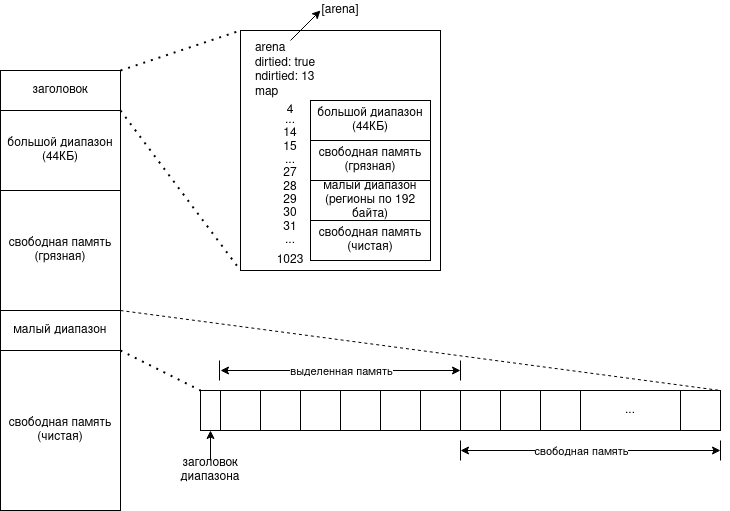
\includegraphics[scale=0.6]{images/jemalloc-arena-chunk.png}
		\caption{Вид блока арены в библиотеке jemalloc.}
		\label{jemalloc-arena-chunk}
	\end{center}
\end{figure}

Каждый фрагмент арены содержит метаданные (в основном карту страниц), за которыми следует один или несколько диапазонов страниц. Небольшие объекты группируются вместе с дополнительными метаданными в начале каждого диапазона страниц, в то время как большие объекты независимы друг от друга, и их метаданные полностью находятся в заголовке блока арены. Каждая арена отслеживает неполную страницу малого объекта через красно-черные деревья (по одному для каждого класса размера), и всегда обслуживает запросы на выделение, используя неполную страницу с наименьшим адресом для этого размерного класса. Каждая арена отслеживает доступную страницу через два красно-черных дерева — одно для чистых/нетронутых страниц и одно для грязных/тронутых страниц. Диапазоны страниц предпочтительно выделяются из грязного дерева с использованием наименьшего наилучшего соответствия.

\begin{figure}[!h]
	\begin{center}
		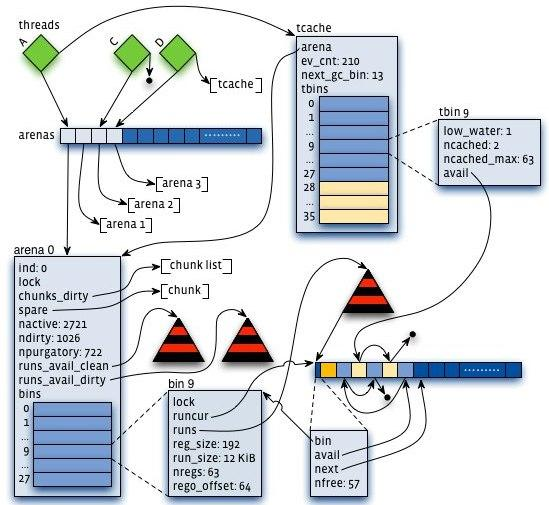
\includegraphics[scale=0.6]{images/jemalloc-arena-and-thread-cache-layout.jpg}
		\caption{Вид арены и потокового кэша в библиотеке jemalloc.}
		\label{jemalloc-arena-and-thread-cache-layout}
	\end{center}
\end{figure}

Каждый поток поддерживает кэш небольших объектов, а также больших объектов до ограниченного размера (по умолчанию 32 КБ). Таким образом, подавляющее большинство запросов на выделение сначала проверяют наличие кэшируемого объекта, прежде чем обращаться к арене. Распределение через кэш потоков не требует никакой блокировки, в то время как распределение через арену требует блокировки ячейки арены (по одной на класс малого размера) и/или арены в целом.

Основная цель потоковых кэшей (или кэшей на каждый процессор) - уменьшить объем событий синхронизации. Таким образом, максимальное количество кэшируемых объектов для каждого размерного класса ограничено на уровне, который позволяет на практике сократить синхронизацию в 10-100 раз. Более высокие ограничения кэширования еще больше ускорят выделение ресурсов для некоторых приложений, но в общем случае это приведет к неприемлемым затратам на фрагментацию. Чтобы еще больше ограничить фрагментацию, кэши выполняют инкрементную "сборку мусора" (GC), где время измеряется в терминах запросов на выделение. Закэшированные объекты, которые остаются неиспользуемыми для одного или нескольких проходов GC, постепенно сбрасываются на соответствующие арены с использованием экспоненциального подхода распада.

\section{Mimalloc}
\textbf{Mimalloc} - это аллокатор, созданный командой исследователей из компании \textit{Microsoft}, для управления выделением и освобождением памяти в функциональных языках программирования таких как \textit{Lean} и \textit{Koka}. В функциональных языках программирования используется подсчет ссылок для управления временем жизни объекта и  создается множество малых объектов. Эти два типа использования приводили к некоторым проблемам с текущими библиотеками. \cite{mimalloc-tech-report}

Прежде всего, и \textit{Lean}, и \textit{Koka} являются функциональными языками, которые выполняют множество небольших кратковременных аллокаций. Кроме того, использование пользовательского аллокатора для таких небольших распределений превзошло даже такие высокооптимизированные библиотеки, как jemalloc. Во-вторых, как и Swift и Python, система выполнения использует подсчет ссылок для управления памятью. Чтобы ограничить паузы при выделении больших структур данных, необходимо поддерживать отложенное уменьшение количества ссылок. Поэтому требуется сотрудничество со стороны самого аллокатора, так как лучшее время для возобновления отложенного декремента – это когда есть нехватка памяти.

В \textbf{mimalloc} используется несколько новых идей, которые помогают библиотеке достичь отличной производительности:
\begin{itemize}
	\item Основная идея состоит в том, чтобы использовать разделение свободных списков: вместо одного большого списка под каждый размерный класс, используется список под страницу в \textbf{mimalloc} (обычно 64 КБ). Это позволяет сохранить локальность выделений внутри одной страницы до тех пор, пока эта страница не будет заполнена, независимо от того, где другие объекты освобождаются в куче;
	\item Использование конкурентных свободных списков, чтобы другие потоки могли освобождать память без синхронизаций. Эти списки также разделены постранично, что помогает избежать конфликтов за ресурсы между ними. Такой список перемещается в локальный свободный список атомарно время от времени, это позволяет эффективно группировать операции освобождения памяти;
	\item Наконец, используется третий локальный свободный список под каждую страницу для локальных освобождений каждого потока. Когда основной свободный список опустошается, локальный список становится новым свободным списком. Такая конструкция гарантирует, что общий путь распределения всегда выбирается после фиксированного количества аллокаций, устанавливая некий временный темп. Теперь эту процедуру можно использовать для амортизации более дорогостоящих операций: освобождение отложенных декрементирований количества ссылок, поддержание детерменированного состояния системы, сбор конкурентных свободных списков под каждый поток. Использование отдельного локального списка позволяет выполнять только одну проверку при выделении памяти быстрым путем, чтобы обрабатывать все вышеперечисленные сценарии через общую процедуру сбора;
	\item Библиотека высоко оптимизирует общие пути распределения и свободного кода, а в других случаях переходит к общей подпрограмме. Это означает, что структуры данных должны быть очень регулярными, чтобы минимизировать условные обозначения в быстром пути. Этот последовательный дизайн также уменьшает количество особых случаев и увеличивает повторное использование кода, что приводит к более регулярному и простому коду;
	\item Блокировок нет, и все взаимодействие между потоками выполняется с использованием атомарных операций.
\end{itemize}

Исторически дизайн аллокаторов был сосредоточен на проблемах производительности, таких как сокращение времени в самом коде аллокатора, сокращение использования памяти или масштабирование до множества параллельных потоков. Реже дизайн мотивируется улучшением локализации ссылок приложения. Например, VAM и ранние версии PHKmalloc также используют сегментацию свободных списков, чтобы гарантировать, что последовательные распределения часто поступают с одной и той же страницы. \textbf{Mimalloc} улучшает локальность ссылок на память приложений и улучшает VAM, реализуя многопоточность и добавляя дополнительные сегментированные свободные списки для уменьшения конкуренции и поддержки амортизирующих задач обслуживания. Такой дизайн демонстрирует, что аллокаторы, ориентированные на улучшение локальной памяти приложений, также могут обеспечить высокую производительность и параллельную масштабируемость.

\subsection{Сегментация свободных списков}
\textit{\textbf{Основной свободный список}}

Шаблон выделения памяти для функционального программирования заключается в выделении и освобождении множества небольших объектов. Многие библиотеки используют один свободный список для каждого размерого класса, что может привести к плохой пространственной локализации, когда объекты, принадлежащие к одной структуре, могут быть распределены по всей куче. Например: в начальном состоянии на рисунке \ref{mimalloc-free-list-state-a}, где свободный список располагается по всему адресному пространству кучи. Если делать запросы на выделение памяти, то состояние переходит к виду как показано на рисунке \ref{mimalloc-free-list-state-b}, где список также располагается по всему адресному пространству кучи с плохой локальностью пространства. Такая ситуация довольно частая, состояние кучи в функциональных языках программирования обычно имеет такой вид. Это происходит, в частности, при сворачивании старых структур данных и создании новых структур данных другого размера, где чередующиеся распределения приводят к таким распределенным свободным спискам.

\begin{figure}[!h]
	\begin{center}
		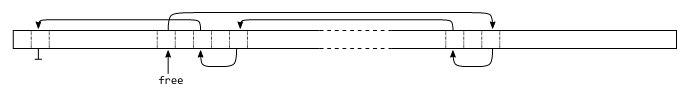
\includegraphics[scale=0.8]{images/mimalloc-free-list-state-a.jpg}
		\caption{Начальное сотояние кучи.}
		\label{mimalloc-free-list-state-a}
	\end{center}
\end{figure}

\begin{figure}[!h]
	\begin{center}
		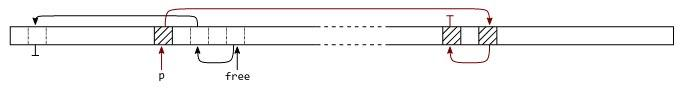
\includegraphics[scale=0.8]{images/mimalloc-free-list-state-b.jpg}
		\caption{Состояние кучи после выделений.}
		\label{mimalloc-free-list-state-b}
	\end{center}
\end{figure}

Чтобы улучшить пространственную локальность распределения, \textbf{mimalloc} использует сегментирование свободных списков, где куча разделена на страницы (по размерным классам) со сводобобным списком под каждую страницу (страницы обычно имеют размер в 64 КБ для малых объектов). Теперь куча будет выглядеть следующим образом, как показано на рисунке \ref{mimalloc-free-list-state-aa}, где каждая страница имеет свой небольшой свободный список:

\begin{figure}[!h]
	\begin{center}
		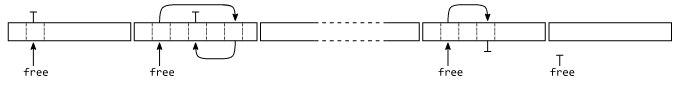
\includegraphics[scale=0.8]{images/mimalloc-free-list-state-aa.jpg}
		\caption{Начальное сотояние кучи.}
		\label{mimalloc-free-list-state-aa}
	\end{center}
\end{figure}

После выделения нескольких объектов, куча переходит в состояние как на рисунке \ref{mimalloc-free-list-state-bb}, где все объекты выделены в рамках одной страницы, что повышает локальность объектов.

\begin{figure}[!h]
	\begin{center}
		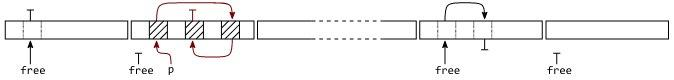
\includegraphics[scale=0.8]{images/mimalloc-free-list-state-bb.jpg}
		\caption{Состояние кучи после выделений.}
		\label{mimalloc-free-list-state-bb}
	\end{center}
\end{figure}

Такой дизайн позволяет библиотеке достичь хорошего времени работы за счет снижения промахов процессорных кешей.

\bigbreak
\textit{\textbf{Локальный свободный список}}

Чтобы связать время освобождения и выделения в наихудшем сценарии, а именно, при освобождении больших структур даных, количетсво рекурсивных вызовов должжно быть оганичено. Среды исполнения для языков программирования обычно используют подсчет ссылок, а ограничение количества вызовов на освобождение памяти с подсчетом ссылок может быть реализовано через счетчик лимита и помещения оставшихся указаьелей в список отложенных декрементов.

Для того чтобы выполнить операцию освобождения для списка декрементов, необходима помощь самого аллокатора, потому что лучшее для этого время это когда аллокатор под нагрузкой и необходимо найти больше свободного места. \textbf{Mimalloc} вызывает пользовательскую процедуру, которая реализуется через обрытный вызов в \textit{deferred\_free}. Она вызывается в медленном пути выделения памяти в процедуре \textit{malloc\_generic} тогда, когда локальный список пуст.

Однако это еще не совсем работает, так как нет никакой гарантии, что общая процедура вызывается регулярно: пользователь может освобождать и выделять несколько раз в пределах одной страницы, при этом свободный список на странице никогда не становится пустым. Вместо этого необходимо убедиться, что общая процедура вызывается после некоторого фиксированного количества выделений. Поэтому список свободных объектов разделяется еще раз: добавляется разделенный список свободных объектов на каждую страницу и пока выделение объектов происходит из обычного списка свободных объектов, любые освобожденные объекты помещаются в локальный список свободных объектов. Это гарантирует, что свободный список станет пустым после фиксированного количества выделений. Теперь можно просто переместить локальный список свободных в список свободных и продолжать выделять:

\begin{lstlisting}
page->free = page->local_free;
page->local_free = NULL;
\end{lstlisting}

Стоит обратить внимание, что не нужно было добавлять условие в быстрый путь для этой ситуации и переводить работу в медленный путь. Теперь, когда \textit{deferred\_free} гарантированно вызывается регулярно после ограниченного числа выделений, можно использовать его в качестве детерминированного контроля состояния аллокатора.

\bigbreak
\textit{\textbf{Конкурентный свободный список}}

В \textbf{mimalloc} страницы принадлежат локальной куче потока, и выделение всегда выполняется в локальной куче. Таким образом, не требуется никаких блокировок. Тем не менее, любой поток может освободить объект. Чтобы избежать блокировок и для локальных освобождений потоков, надо добавить конкурентный список свободных объектов на страницу, куда другие потоки смогут освобождать объекты в этой странице. Если происходит освобождение памяти из другого потока, используется атомарная операция для помещения объекта в список:

\begin{lstlisting}
atomic_push( &page->thread_free, p );

void atomic_push( block_t** list, block_t* block ) {
	do {
		block->next = *list;
	}while (!atomic_compare_and_swap(list, block, block->next));
}
\end{lstlisting}

Суть конкурентного списква в том, что он понижает соревнование между потоками, потому что потоки, освобождающие объекты в разных страницах, не соревнуются друг с другом. В современных архитектурах несогласованные атомарные операции очень эффективны и обычно реализуются как часть протокола когерентности кэша.

Чтобы добавить свободную память конкурентного списка в общий, используется следуюая последовательность вызовов:
\begin{lstlisting}
tfree = atomic_swap( &page->thread_free, NULL );
append( page->free, tfree );
\end{lstlisting}

Так как целый список перемещается сразу, то нелокальные вызовы осбобождения памяти тоже эффективно группируются. Это очень важно для асимметричных параллельных рабочих нагрузок где множество потоков периодически освобождают объекты, а другие выделяют.

\subsection{Реализация}

\bigbreak
\textit{\textbf{Выделение памяти}}

\begin{figure}[!h]
	\begin{center}
		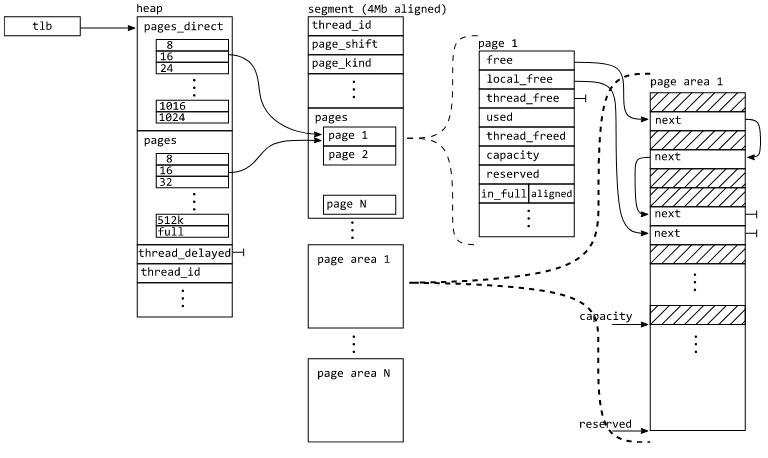
\includegraphics[scale=0.8]{images/mimalloc-design-overview.jpg}
		\caption{Компоновка кучи.}
		\label{mimalloc-design-overview}
	\end{center}
\end{figure}

Для выделения объекта, библиотека сначала получает доступ к указателю на локальную для потока кучу (tlb). Далее идет поиск страницы нужного размерного класса. Для малых объектов, размер которых менее чем 1 КБ, куча содержит массив указателей на первую свободную страницу в каждом размерном классе.

\pagebreak

\begin{lstlisting}
void* malloc_small( size_t n ) {                    // 0 < n <= 1024
	heap_t*  heap  = tlb;
	page_t*  page  = heap->pages_direct[(n+7)>>3];
	block_t* block = page->free;
	if (block==NULL) return malloc_generic(heap,n);
	page->free = block->next
	page->used++;
	return block;
}
\end{lstlisting}

Как можно увидеть на рисунке \ref{mimalloc-design-overview}, сами страницы и их метаданные находятся в больших сегментах памяти (слаб или арена). Размер такой арены - 4 МБ (или больше для объектов, размер которых более 512 КБl), Есть три класса размеров страниц: 64 КБ для объектов, которые меньше чем 8 КБ, 4 МБ для объектов, которые меньше чем 512 КБ и для объектов, которые больше чем 512 КБ, размер страницы равен запрашиваемому размеру самого объекта.

\bigbreak
\textit{\textbf{Освобождение памяти}}

Страницы и их метаданные выделяются в одном сегменте для того, чтобы снизить дорогие системные вызовы ОС, но есть еще одна веская причина: при освобождении указателя, надо найти метаданные страницы, к которым принадлежит этот указатель. В \textbf{mimalloc} это реализовано путем выравнивания сегментов по адресам кратным 4 МБ. Благодаря этому можно получить сегмент, содержащий указатель умножением нижних битов указателя и маски.

\begin{lstlisting}
void free( void* p ) {
	segment_t* segment = (segment_t*)((uintptr_t)p & ~(4*MB));
	if (segment==NULL) return;
	page_t*    page    = &segment->pages[(p - segment) >> segment->page_shift];
	block_t*   block   = (block_t*)p;
	if (thread_id() == segment->thread_id) {
		block->next = page->local_free;
		page->local_free = block;
		page->used--;
		if (page->used - page->thread_freed == 0) page_free(page);
	}else {
		atomic_push( &page->thread_free, block);
		atomic_incr( &page->thread_freed );
	}
}
\end{lstlisting}

Процедура освобождения сначала получает указатель на сегмент путем маскирования нижних битов освобождаемого указателя. Далее можно вычислить индекс страницы через разницу между указателем и сегментом и сдвигая биты на смещение: для малых объектов оно равно 16 (64 КБ), тогда как для больших 22 (4 МБ). После выполняется проверка на то, в какой список поместить освобожденный объект, локальный или конкурентный. Тут \textbf{mimalloc} полагается на вызов функции \textit{thread\_id()} для получения идентификатора текущего потока и далее сравнивая его с переменной \textit{thread\_id} сегмента.

Если функция \textit{free} была вызвана из другого потока, то объект атомарно помещается в конкурентный список. Иначе, освобождение локально для текущего потока и объект помещается в локальный для потока список. Если в процессе освобождения указателя страница становится пустой, она тоже освобождается. Этот шаг можно пропустить и накапливать пустые страницы, но это может ухудшить ситуацию а том случае, если программа редко выделяет большой объем памяти и потом быстро его освобождает.

\bigbreak
\textit{\textbf{Общее выделение памяти}}

Обобщенный случай выделения памяти описывается процедурой \textit{malloc\_generic}, которая гарантированно вызывается время от времени. Эта процедура позволяет амортизировать сложные операции и выполняет роль сборщика мусора.

\begin{lstlisting}
void* malloc_generic( heap_t* heap, size_t size ) {
	deferred_free();
	foreach( page in heap->pages[size_class(size)] ) {
		page_collect(page);
		if (page->used - page->thread_freed == 0) {
			page_free(page);
		}else if (page->free != NULL) {
			return malloc(size);
		}
	}
	...
}

void page_collect(page) {
	page->free = page->local_free;
	page->local_free = NULL;
	...
}
\end{lstlisting}

Процедурп проходит по всем страницам размерного класса и освобождает те, которые пустые. Она останавливается когда находит первую частично занятую страницу с пустыми объектами. Не все страницы сразу освобождаются, неоторые остаются закэшированными в случае если они могут вскоре понадобиться. Максимальное количество освобождаемых страниц лимитировано, чтобы снизить количество наихудших случаев при выделении памяти. Если полученная страница находилась в свободном списке, список ротируется и новый поиск начинается со следующей страницы.

\bigbreak
\textbf{\textit{Полный список}}

Изначально \textbf{mimalloc} плохо работал с типами выделений памяти, когда программа использовала свои самописные аллокаторы и запрашивала много большое количество памяти в самом начале своего исполнения и такие объекты оставались в используемом состоянии на протяжении времени работы программы. Поэтому был реализован одельный полный список, который содержит заполненные страницы. Если объекты в таких страницах освобождаются, то они помещаются в обычные списки. Но такое изменение вносит усложнение для многопоточных случаев.

В случае когда освобождается объект из полного списка из другого потока, надо сигнализировать куче о том, что страница больше не полная, при этом делать это без блокировок. Это реализовано через отдельный конкурентный список отложенных освобождений. Вначале функции \textit{free} идет итерация по этому списку и освобождаются все объекты в нем, попутно объекты перемещаются в обычные списки, если это возможно.

Чтобы это работало, функция должна знать в каком случае надо вставить в конкурентеый список отложенных освобождений или в обычный конкурентный список. Для этого используются два нижних бита в указателе на конкурентный список, которые задают 3 состояния: NORMAL, DELAYED и DELAYING. В обычном случае состояние имеет тип NORMAL и все освобождаемые объекты помещаются в локальный конкурентный список. Когда страница помещается в полный список, состояние устанавливается в DELAYED, которое говорит о том, что другие потоки должны помещать удаляемые объекты в конкурентный список отложенных освобождений. Пока это вполняется, состояние временно выставляется в DELAYING, чтобы гарантировать достоверное состояние куче, если поток, который ей управляет, вдруг уничтожается. Псоле отложенного освобождения состояние вновь выставляется в NORMAL, потому что нужно только одно отложенное освобождение, чтобы проверить что страница больше не заполнена. Это довольно важное улучшение: при асимметричных рабочих нагрузках, освобождающий поток может освободить много объектов и надо удостовериться что список отложенный удалений проверяется только один раз.

\begin{figure}[!h]
	\begin{center}
		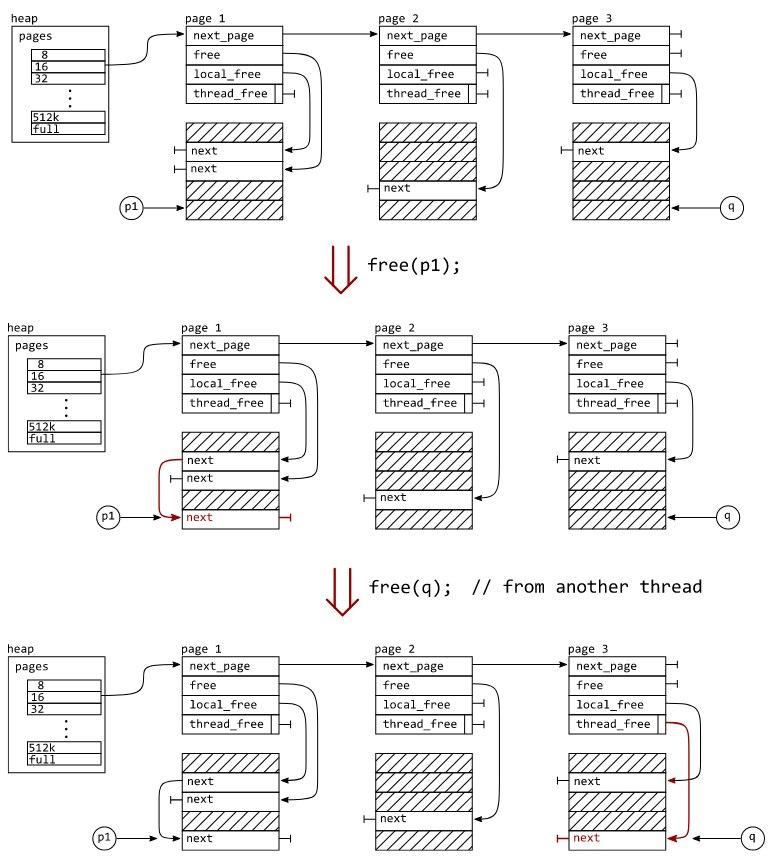
\includegraphics[scale=0.5]{images/mimalloc-free.jpg}
		\caption{Освобождение объектов.}
		\label{mimalloc-free}
	\end{center}
\end{figure}

\begin{figure}[!h]
	\begin{center}
		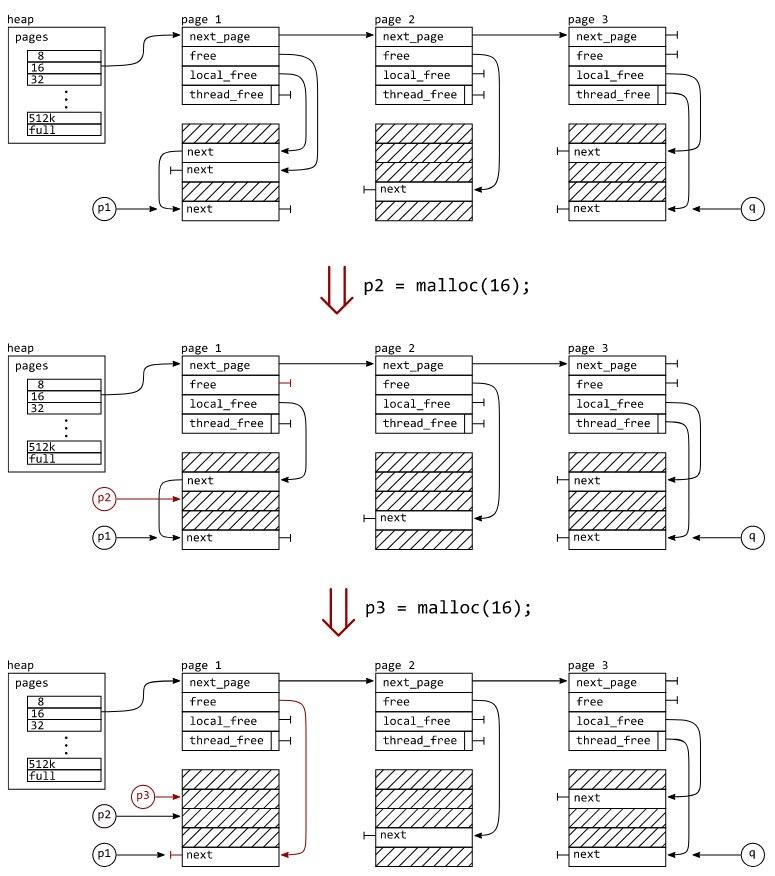
\includegraphics[scale=0.5]{images/mimalloc-alloc.jpg}
		\caption{Выделение объектов.}
		\label{mimalloc-alloc}
	\end{center}
\end{figure}

\section{Rpmalloc}\bigbreak

Аллокатор был разработан Маттиасом Янссоном (Mattias Jansson) в компании Rampant pixels. Он похож на \textbf{Tcmalloc} и использует отдельные кучи для каждого потока и разбивает блоки памяти в соответствии с предварительно настроенным набором классов размероми до 2 МБ. Более крупные блоки выделяются и освобождаются прямо в ОС. Запросы на выделение памяти для разных размерных классов обслуживаются из разных наборов страниц памяти, каждый диапазон страниц посвящен одному размерному классу. Диапазоны страниц могут передаваться между потоками, когда кэш потоков переполняется и освобождается в глобальный кэш, или когда поток заканчивает исполнение. В отличие от \textbf{Tcmalloc}, отдельные блоки не перемещаются между потоками, а только целые диапазоны страниц.\cite{rpmalloc}

\bigbreak
\textit{\textbf{Детали реализации}}
	
Библиотека основана на фиксированном, но настраиваемом выравнивании страниц (по умолчанию 64 КБ) и выравнивании блоков 16 байт, где все спаны сопоставляются с этой границей выравнивания. В Windows это автоматически гарантируется до 64 Кб за счет детализации VirtualAlloc, а в системах mmap это достигается за счет увеличения размера отображения и выравнивания возвращаемого адреса виртуальной памяти до требуемых границ. Благодаря выравниванию по фиксированному размеру, операция освобождения может найти заголовок области памяти без необходимости поиска по таблице (как это делает \textbf{Tcmalloc}), просто маскируя младшие биты адреса (для 64 КБ это младшие 16 бит).

Блоки памяти делятся на три категории. Для размера/выравнивания интервала 64 Кб малые блоки составляют [16, 1024] байт, средние блоки (1024, 32256] байт и большие блоки (32256, 2097120] байт. Эти три категории далее разделены по классам размеров. Если размер промежутка изменяется, классы малых блоков остаются, но средние блоки идут от (1024, размер промежутка] байт.

Гранулярность малых блоков состовляет 16 байт и таких всего 64 типа. Средние блоки имеют гранулярность 512 байт, их 61 (по умолчанию). Большие блоки имеют ту же степень гранулярности, что и настроенный размер спана (по умолчанию 64 Кб). Все выделения соответствуют этим границам (выделение в 36 байт выделит блок в 48 байт). Каждый класс малого и среднего размера имеет связанную конфигурацию диапазонов (то есть непрерывный набор страниц памяти), описывающую, сколько страниц будет выделяться классом размера каждый раз, когда кэш пуст и запрашивается новое выделение.

Каждый диапазон для классов малого и среднего размеров отслеживает, сколько блоков выделено/свободно, а также список блоков, которые свободны для выделения. Чтобы избежать блокировок, каждый спан полностью принадлежит выделяющему потоку, и все межпотоковые освобождения будут отложены для потока-владельца через отдельный свободный список для каждого диапазона.

Большие блоки или суперспаны, кэшируются на двух уровнях. Первый уровень - это список свободных суперспанов для каждого потока. Второй уровень - это глобальный список свободных суперспанов.

\bigbreak
\textit{\textbf{Отображение памяти}}

По умолчанию аллокатор использует API ОС для выделения страниц виртуальной памяти по мере необходимости, либо VirtualAlloc в Windows, либо mmap в системах POSIX. Если надо хотит использовать свою собственную реализацию сопоставления памяти из ядра в пространство пользователя, можно использовать \textit{rpmalloc\_initialize\_config }и передавать указатели функций для отображения и снятия отображения виртуальной памяти. Эти функции должны резервировать и освобождать запрошенное количество байтов.

Возвращаемый адрес памяти из функции отображения памяти должен быть выровнен по размеру страницы памяти и размеру области памяти (который всегда больше), оба из которых настраиваются. Либо можно указать размеры страницы и интервала во время инициализации с помощью \textit{rpmalloc\_initialize\_config}, либо использовать \textit{rpmalloc\_config}, чтобы найти требуемое выравнивание, равное максимальному размеру страницы и интервалу. Размер диапазона должен быть в степени двойки в диапазоне [4096, 262144] и быть кратным или делителем размера страницы памяти.

Запросы на отображение памяти всегда выполняются в кратных размерах страницы памяти. Можно указать пользовательский размер страницы при инициализации \textbf{rpmmalloc} с помощью \textit{rpmalloc\_initialize\_confi}g или передать 0, чтобы \textbf{rpmalloc} определял размер страницы системной памяти с помощью API ОС. Размер страницы должен быть кратен степени двойки.

Чтобы уменьшить накладные расходы на системные вызовы, спаны отображаются пачками, управляемыми переменной конфигурации \textit{span\_map\_count} (по умолчанию значение \textit{DEFAULT\_SPAN\_MAP\_COUNT} равно 0, размер которого, в свою очередь, определяется в соответствии с определением конфигурации кэша, по умолчанию равным 64). Если размер страницы памяти больше размера спана, количество спанов для отображения в одном вызове будет скорректировано, чтобы гарантировать кратность размера страницы, и спаны будут отображаться до тех пор, пока весь диапазон не будет размечен одним вызовом (чтобы избежать попыток размечения частичных страниц).

\bigbreak
\textit{\textbf{Большие сраницы}}

Аллокатор поддерживает большие страницы в Windows, Linux и macOS. Для использования надо передать ненулевое значение в конфигурационном значении \textit{enable\_huge\_pages} при инициализации аллокатора с помощью \textit{rpmalloc\_initialize\_config}. Если система не поддерживает большие страницы, опция не будет использоваться. Можно запросить статус, посмотрев на \textit{enable\_huge\_pages} в конфигурации, возвращенной после вызова \textit{rpmmalloc\_config} после завершения инициализации.

\bigbreak
\textit{\textbf{Разрыв диапазонов}}

Суперспаны (несколько спанов, идущих подряд) могут быть разделены на меньшие диапазоны, чтобы удовлетворить потребность в отображении нового диапазона памяти. По умолчанию аллокатор будет жадно захватывать и разрывать любой больший промежуток из доступных кэшей, прежде чем отображать новую виртуальную память. Однако в настоящее время спаны не могут быть склеены вместе, чтобы снова сформировать большие суперпролеты. Подпространства могут пересекать кэш и использоваться различными потоками по отдельности.

Спан, который является подпространством большего суперпространства, может быть индивидуально списан, чтобы уменьшить нагрузку на физическую память, когда спан будет удален из кэшей и запланирован для отмены отображения. Весь исходный суперспан будет отслеживать подпространства, на которые он разбит, и когда весь диапазон будет выведен из эксплуатации, его отображение будет отменено. Это позволяет платформам, таким как Windows, для которых требуется, чтобы весь диапазон виртуальной памяти, отображенный при вызове VirtualAlloc, был отменен при одном вызове VirtualFree, при этом отдельные страницы в подпространствах (если размер страницы меньше, чем размер спана) будут удалены.

Если bcgjkmpetncz пользовательская функция отображения памяти, необходимо это учитывать, за это отвечает параметр \textit{release}, передаваемый функции \textit{memory\_unmap}. Он равен 0 в случае списания отдельных страниц и общему размеру суперпространства в байтах для окончательного освобождения всего диапазона памяти суперпространства.

\bigbreak
\textit{\textbf{Фрагментация памяти}}

Библиотека не оставляет нераспределенные и непригодные для использования фрагменты на страницах памяти при вызовах выделения и освобождения блоков разных размеров. Это связано с тем, что страницы памяти, выделенные для каждого размерного класса, разбиты на идеально выровненные блоки, которые не используются повторно для запроса другого размера. Блок, освобожденный вызовом \textit{free}, всегда будет немедленно доступен для запроса на выделение в том же размерном классе.

Однако существует фрагментация памяти в том смысле, что запрос на \textbf{N} байтов, за которым следует запрос на \textbf{M} байтов, где N и M имеют разные классы размеров, вернет блоки, разделенные по крайней мере одной страницей памяти в виртуальном адресном пространстве. Только блоки одинакового размера потенциально будут находиться в пределах одного и того же диапазона страниц памяти.

\textbf{rpmalloc} сохраняет "активный диапазон" и свободный список для каждого класса размеров. Это приводит к тому, что последовательные выделения, скорее всего, будут обслуживаться из одного и того же промежутка страниц памяти (если только в этом промежутке не закончатся свободные блоки). Реализация \textbf{rpmalloc} также будет использовать любые фрагменты в страницах памяти в полупустых промежутках, прежде чем использовать полностью свободный промежуток.

\bigbreak
\textit{\textbf{Кучи первого класса}}

\textbf{rpmmalloc} предоставляет тип кучи первого класса с явным API управления кучей. Кучи поддерживаются с помощью вызовов \textit{rpmalloc\_heap\_acquire} и \textit{rpmalloc\_heap\_release}, а выделение/освобождение выполняется с помощью \textit{rpmalloc\_heap\_alloc} и \textit{rpmalloc\_heap\_free}. Основной вариант использования явного управления кучей состоит в том, чтобы ограничить выделения в куче и освободить всё с помощью одного вызова \textit{rpmalloc\_heap\_free\_all} без необходимости поддерживать владение блоками памяти. API кучи не является потокобезопасным, пользователь должен убедиться, что каждая куча используется только в одном потоке в любой момент времени.

\section{Выводы}
В результате сравнения различных методов распределения памяти показано, что метод, реализуемый библиотекой tcmalloc, является лучшим. Этот метод показывает хорошую скорость исполнения запросов на распределение памяти, при этом имея достаточно низкий процент накладных расходов.

Отличительной особенностью данного метода является возможность переиспользования потоковых кэшей для малых объектов другими потоками. Для каждого логического процессора имеется свой кэш, который обеспечивает данным локальность, а сама ОС старается исполнять потоки на тех же процессорах, чтобы минимизировать накладные расходы на копирование. При этом, доступ к кэшам контролируется через вызов \textit{rseq}, который является программной реализацией транзакционной памяти. Запрос на запись проходит полностью или начинается с самого начала последовательности. Благодаря этому не нужно синхронизировать доступ к ресурсам, что снижает накладные расходы на чтение и запись.

\begin{table}[]
	\caption{Распределение памяти для размеров [16, 1000]}
	\resizebox{\columnwidth}{!}{%
	\begin{tabular}{|c|c|c|c|c|}
		\hline
		Аллокатор    & \begin{tabular}[c]{@{}c@{}}Количество операций\\ в секунду\end{tabular} & \begin{tabular}[c]{@{}c@{}}Запрошенная память\\ (МБ)\end{tabular} & \begin{tabular}[c]{@{}c@{}}Выделенная память\\ (МБ)\end{tabular} & \begin{tabular}[c]{@{}c@{}}Накладные расходы\\ (\%)\end{tabular} \\ \hline
		glibc malloc & 1164848                                                                 & 274.45                                                            & 436.91                                                           & 37.18                                                            \\ \hline
		tcmalloc     & 1528605                                                                 & 266.81                                                            & 360.23                                                           & 25.93                                                            \\ \hline
		jemalloc     & 1390639                                                                 & 275.96                                                            & 445.71                                                           & 38.09                                                            \\ \hline
		mimalloc     & 1717668                                                                 & 259.49                                                            & 474.61                                                           & 45.33                                                            \\ \hline
		rpmalloc     & 1738341                                                                 & 262.34                                                            & 576.54                                                           & 54.5                                                             \\ \hline
	\end{tabular}%
}
\end{table}

\begin{table}[]
	\caption{Распределение памяти для размеров [16, 8000]}
	\resizebox{\columnwidth}{!}{%
	\begin{tabular}{|c|c|c|c|c|}
		\hline
		Аллокатор    & \begin{tabular}[c]{@{}c@{}}Количество операций\\ в секунду\end{tabular} & \begin{tabular}[c]{@{}c@{}}Запрошенная память\\ (МБ)\end{tabular} & \begin{tabular}[c]{@{}c@{}}Выделенная память\\ (МБ)\end{tabular} & \begin{tabular}[c]{@{}c@{}}Накладные расходы\\ (\%)\end{tabular} \\ \hline
		glibc malloc & 1196586                                                                 & 344.37                                                            & 487.8                                                            & 29.4                                                             \\ \hline
		tcmalloc     & 1617384                                                                 & 332.47                                                            & 500.95                                                           & 33.63                                                            \\ \hline
		jemalloc     & 1511957                                                                 & 341.39                                                            & 517.58                                                           & 34.04                                                            \\ \hline
		mimalloc     & 1768931                                                                 & 330.46                                                            & 540.15                                                           & 38.82                                                            \\ \hline
		rpmalloc     & 1806651                                                                 & 359.02                                                            & 1390.66                                                          & 74.18                                                            \\ \hline
	\end{tabular}%
}
\end{table}

\begin{table}[]
	\caption{Распределение памяти для размеров [16, 16000]}
	\resizebox{\columnwidth}{!}{%
	\begin{tabular}{|c|c|c|c|c|}
		\hline
		Аллокатор    & \begin{tabular}[c]{@{}c@{}}Количество операций\\ в секунду\end{tabular} & \begin{tabular}[c]{@{}c@{}}Запрошенная память\\ (МБ)\end{tabular} & \begin{tabular}[c]{@{}c@{}}Выделенная память\\ (МБ)\end{tabular} & \begin{tabular}[c]{@{}c@{}}Накладные расходы\\ (\%)\end{tabular} \\ \hline
		glibc malloc & 427880                                                                  & 1398.01                                                           & 2006.45                                                          & 30.32                                                            \\ \hline
		tcmalloc     & 447752                                                                  & 1434.6                                                            & 1832.22                                                          & 21.7                                                             \\ \hline
		jemalloc     & 446116                                                                  & 1418.47                                                           & 2089.75                                                          & 32.12                                                            \\ \hline
		mimalloc     & 512712                                                                  & 1348.06                                                           & 2072.96                                                          & 34.97                                                            \\ \hline
		rpmalloc     & 540037                                                                  & 1525.17                                                           & 7253.42                                                          & 78.97                                                            \\ \hline
	\end{tabular}%
}
\end{table}

\begin{table}[]
	\caption{Распределение памяти для размеров [128, 64000]}
	\resizebox{\columnwidth}{!}{%
	\begin{tabular}{|c|c|c|c|c|}
		\hline
		Аллокатор    & \begin{tabular}[c]{@{}c@{}}Количество операций\\ в секунду\end{tabular} & \begin{tabular}[c]{@{}c@{}}Запрошенная память\\ (МБ)\end{tabular} & \begin{tabular}[c]{@{}c@{}}Выделенная память\\ (МБ)\end{tabular} & \begin{tabular}[c]{@{}c@{}}Накладные расходы\\ (\%)\end{tabular} \\ \hline
		glibc malloc & 397210                                                                  & 1243.05                                                           & 1527.54                                                          & 18.62                                                            \\ \hline
		tcmalloc     & 400676                                                                  & 1222.46                                                           & 1598.48                                                          & 23.52                                                            \\ \hline
		jemalloc     & 289433                                                                  & 1191.81                                                           & 1716.3                                                           & 30.56                                                            \\ \hline
		mimalloc     & 419151                                                                  & 1057.64                                                           & 1747.74                                                          & 39.49                                                            \\ \hline
		rpmalloc     & 453496                                                                  & 1202.48                                                           & 9568.01                                                          & 87.43                                                            \\ \hline
	\end{tabular}%
}
\end{table}

\begin{table}[]
	\caption{Распределение памяти для размеров [512, 160000]}
	\resizebox{\columnwidth}{!}{%
	\begin{tabular}{|c|c|c|c|c|}
		\hline
		Аллокатор    & \begin{tabular}[c]{@{}c@{}}Количество операций\\ в секунду\end{tabular} & \begin{tabular}[c]{@{}c@{}}Запрошенная память\\ (МБ)\end{tabular} & \begin{tabular}[c]{@{}c@{}}Выделенная память\\ (МБ)\end{tabular} & \begin{tabular}[c]{@{}c@{}}Накладные расходы\\ (\%)\end{tabular} \\ \hline
		glibc malloc & 179929                                                                  & 1856.5                                                            & 2546.84                                                          & 27.11                                                            \\ \hline
		tcmalloc     & 173264                                                                  & 2101.51                                                           & 2672.14                                                          & 21.35                                                            \\ \hline
		jemalloc     & 112656                                                                  & 2029.18                                                           & 2700.34                                                          & 24.85                                                            \\ \hline
		mimalloc     & 173412                                                                  & 2035.98                                                           & 2960.11                                                          & 31.22                                                            \\ \hline
		rpmalloc     & 185280                                                                  & 2015.17                                                           & 14680.04                                                         & 86.27                                                            \\ \hline
	\end{tabular}%
}
\end{table}